 \chapter[Structure with two neutrons]{Structure with transfer}\label{C8}
 In what follows, we apply the formalism worked out in the previous chapters with the help of software developed to calculate absolute one-- and two--particle transfer differential cross sections, to analyze reactions induced by both light and heavy ions (see App. \ref{C8AppD} \textsc{cooper}, \textsc{one}).
 A number of examples are considered covering nuclei throughout the mass table. Namely, one-- and two-- particle transfer reactions on Be--isotopes as well as two--particle transfer on   $^{7}$Li, $^{11}$Li, $^{48}$Ca, and $^{206}$Pb (systems around closed shells), and on open shell superfluid medium heavy nuclei (Sn--isotopes).
 \section[Evidence for phonon mediated pairing]{The $^1$H($^{11}$Li,$^9$Li)$^3$H reaction: evidence for phonon mediated pairing}\label{C8S1}
    \begin{figure}
    \centerline{\includegraphics*[width=16cm,angle=0]{C8/figsC8/fig8_1_3x}}
    	\caption{\emph{Gedanken} (two--particle transfer) coincidence experiments aimed at better individuating the couplings involved in the neutron halo Cooper pair correlations in $^{11}$Li and of the $1/2^-$ first excited state of $^9$Li populated in the  
    	 $^1$H($^{11}$Li,$^9$Li)$^3$H  reaction (\cite{Tanihata:08,Barranco:01,Potel:10}). From \cite{Potel:14}. It is of notice the lack of detail regarding the reaction aspect of the process, to emphasize some structural features.}\label{fig8_1_3}
    \end{figure}
 \begin{figure}
 \centerline{\includegraphics*[width=15cm,angle=0]{C8/figsC8/fig8_1_1}}
 	\caption{Schematic representation of the bare nucleon-nucleon and phonon induced pairing correlations (upper part) NFT diagrams, and of the population of the first, excited state of $^{9}$Li($1/2^{-}; 2.69$ MeV), in the TRIUMF experiment  reported in ref. \cite{Tanihata:08}.}\label{fig8_1_1}
 \end{figure}
 We start by discussing  the analysis of the two--neutron pickup\footnote{\cite{Tanihata:08}.} reaction $^1$H($^{11}$Li,$^9$Li)$^3$H. Particular  attention is paid to the  excitation of the $1/2^-$ first excited state of $^9$Li lying at 2.69 MeV (see Figs. \ref{figintro5} and  \ref{fig8_1_3})\footnote{To assess the direct character of the $1/2^-$ excitation process, the importance of inelastic  and knockout (cf. Ch.\ref{C6}) channels were considered and found to be small (see App. \ref{C8AppB}).}. The results  provide evidence for a new mechanism of pairing correlations in nuclei: pygmy resonance (low--energy $E1$--strength) mediated pairing interaction\footnote{\citet{Barranco:01,Potel:10}.}, which strongly renormalizes the bare, $NN$--$^1S_0$ interaction. This is but a particular embodiment of phonon mediated pairing interaction found throughout in nuclei\footnote{See e.g. \citet{Barranco:99,Gori:04} cf. also \citet{Brink:05}.}. The main difference between light halo exotic nuclei and medium heavy superfluid nuclei lying along the valley of stability is the role fluctuations play in dressing particles (quasiparticles) and in renormalizing their properties (mass, charge, etc.) and their interactions.
  \begin{figure}
  \centerline{\includegraphics*[width=18cm,angle=0]{C8/figsC8/fig8_1_3}}
  	\caption{Absolute, two--nucleon transfer differential cross section associated with the ground state and the first 	excited state of $^9$Li, excited  in the reaction $^1$H($^{11}$Li,$^9$Li)$^3$H \citep{Tanihata:08} in comparison with the predicted differential cross sections \citep{Potel:10} worked out making use of spectroscopic amplitudes and Cooper pair wavefunctions calculated with NFT, and of the optical potential collected in Table \ref{tab8.1.1}.}\label{fig8_1_2}
  \end{figure}
 In fact, in the case of e.g. Sn isotopes, mean field effects are dominant, while in the case of halo exotic nuclei renormalization effects can be as large as mean field ones. Concerning the pairing interaction, bare and induced contributions are about equal in the case of i.e. Sn--isotopes, while the second one is the overwhelming contribution in the case of $^{11}$Li. The collective modes acting as glue of the Cooper pairs are mainly of quadrupole type in Sn and of dipole (pygmy resonance) type in the case of Li. 

 
 
 
 
 
 

\subsection{Structure}
Within the scenario presented in Chapter \ref{chapter1}  (Sect. \ref{App1AF}) and Chapter \ref{C6} (Sect. \ref{C6S2.2x}) the wavefunction describing the structure of the halo neutrons in the ground state of $^{11}$Li (the $p_{3/2}$ proton being assumed to act only as a spectator) can be written as
\begin{equation}\label{eq8_2_1}
|0\rangle_\nu=|0\rangle+\alpha|(p_{1/2},s_{1/2})_{1^-}\otimes 1^-;0\rangle+\beta|(s_{1/2},d_{5/2})_{2^+}\otimes 2^+;0\rangle,
\end{equation}
with
\begin{equation}\label{eq8_2_2}
\alpha=0.7,\quad \text{and} \quad \beta=0.1,
\end{equation}
and
\begin{equation}\label{eq8_2_3}
|0\rangle=0.45|s_{1/2}^2(0)\rangle+0.55|p_{1/2}^2(0)\rangle+0.04|d_{5/2}^2(0)\rangle,
\end{equation}
$|1^-\rangle$ and $|2^+\rangle$ being the (RPA) states describing the dipole pygmy resonance of $^{11}$Li and the quadrupole vibration of the core. The corresponding NFT diagrams are shown in diagrams (a), (d) and (e) of Fig. \ref{figintro5}. The wavy curve represents both the quadrupole and dipole collective vibrational states being exchanged between the two halo neutrons, the horizontal dashed line the bare nuclear pairing interaction.




\begin{table}[h!]
%\caption{Optical model parameters used in the two--neutron transfer calculations}
{\begin{tabular}{|c|c|c|c|c|c|c|c|c|c|c|c|c|}
\cline{2-13} 
\multicolumn{1}{c|}{}& \multicolumn{12}{|c|}{$^{11}$Li($p,t)^{9}$Li}           \\
\cline{2-13} 
\multicolumn{1}{c|}{} & $V$ & $W$ &  $V_{so}$ &  $W_d$ &  $r_1$ &  $a_1$ &  $r_2$ &  $a_2$ &  $r_3$ &  $a_3$ &  $r_4$ &  $a_4$            \\
\hline 
$p$,\;$^{11}$Li$\,^{d)}$ & $63.62$ & $0.33$ &  $5.69$ &  $8.9$ &  $1.12$ &  $0.68$ &  $1.12$ &  $0.52$ &  $0.89$ &  $0.59$ &  $1.31$ &  $0.52$ \\
\hline 
$d$,\;$^{10}$Li$\,^{b)}$ & $90.76$ & $1.6$ &  $3.56$ &  $10.58$ &  $1.15$ &  $0.75$ &  $1.35$ &  $0.64$ &  $0.97$ &  $1.01$ &  $1.4$ &  $0.66$ \\
\hline 
$t$,\;$^{9}$Li$\,^{c)}$ & $152.47$ & $12.59$ &  $1.9$ &  $12.08$ &  $1.04$ &  $0.72$ &  $1.23$ &  $0.72$ &  $0.53$ &  $0.24$ &  $1.03$ &  $0.83$ \\
\hline 

\hline 
  \end{tabular}}
   \caption{Optical potentials (cf. \cite{Tanihata:08}) used in the calculation of the absolute differential cross sections displayed in Fig. \ref{fig8_1_2} and Table \ref{tab6.1.2}.}
\label{tab8.1.1}
\end{table}



\begin{table}[h!]
%\caption{Optical model parameters used in the two--neutron transfer calculations}
{\begin{tabular}{|c|c|c|c|c|c|c|c|c|c|c|c|c|}
\cline{2-13} 
\multicolumn{1}{c|}{}& \multicolumn{12}{|c|}{$^{11}$Li($p,t)^{9}$Li}           \\
\cline{2-13} 
\multicolumn{1}{c|}{} & $V$ & $W$ &  $V_{so}$ &  $W_d$ &  $r_1$ &  $a_1$ &  $r_2$ &  $a_2$ &  $r_3$ &  $a_3$ &  $r_4$ &  $a_4$            \\
\hline 
$p$,\;$^{11}$Li$\,^{d)}$ & $63.62$ & $0.33$ &  $5.69$ &  $8.9$ &  $1.12$ &  $0.68$ &  $1.12$ &  $0.52$ &  $0.89$ &  $0.59$ &  $1.31$ &  $0.52$ \\
\hline 
$d$,\;$^{10}$Li$\,^{b)}$ & $90.76$ & $1.6$ &  $3.56$ &  $10.58$ &  $1.15$ &  $0.75$ &  $1.35$ &  $0.64$ &  $0.97$ &  $1.01$ &  $1.4$ &  $0.66$ \\
\hline 
$t$,\;$^{9}$Li$\,^{c)}$ & $152.47$ & $12.59$ &  $1.9$ &  $12.08$ &  $1.04$ &  $0.72$ &  $1.23$ &  $0.72$ &  $0.53$ &  $0.24$ &  $1.03$ &  $0.83$ \\
\hline 

\hline 
  \end{tabular}}
   \caption{Integrated two--neutron differential cross sections associated with the reaction $^1$H($^{11}$Li,$^9$Li($i$))$^{3}$H populating the ground state and the first excited state of $^{9}$Li (\cite{Tanihata:08}, column labeled Experiment). The theoretical values are from \cite{Potel:10} (see also \cite{Potel:13}). See Figs. \ref{fig8_1_2} and \ref{fig8_B_2}.}
\label{tab6.1.2}
\end{table}




We are then in presence of a paradigmatic nuclear embodiment of Cooper's model which is at the basis of BCS theory: a single weakly bound neutron pair on top of the Fermi surface of the ${}^9$Li core. But the analogy goes beyond these aspects, and covers also the very nature of the interaction acting between Cooper pair partners. Due to the  the high polarizability of the system under study and of the small overlap of halo and core single particle wavefunctions, most of the Cooper pair correlation energy stems, according to NFT, from the exchange of collective vibrations, the role of the strongly screened bare interaction being, in this case, minor and  (see Sect. \ref{App1AF}). In other words, we are in the presence of a new realization of the Cooper model in which a totally novel Bardeen--Pines--Fr\"olich--like phonon induced interaction is generated by a self induced collective vibration of the nuclear medium.



 In connection with  (\ref{eq8_2_1}), it is suggestive that the two states populated in the  inverse kinematics, two--neutron pick up reaction $^1$H($^{11}$Li,$^9$Li)$^3$H are\footnote{\cite{Tanihata:08}.}, the $|3/2^-\text{gs}(^9\text{Li})\rangle$ and the first excited $|1/2^-,2.69\text{MeV}\rangle$ level of $^9$Li  (see Figs. \ref{figintro5} (f) and \ref{fig8_1_3}). In fact, the associated absolute differential cross sections probe, within the NFT scenario, the $|0\rangle$  and the $|(s_{1/2},d_{5/2})_{2^+}\otimes 2^+;0\rangle$ component of the Cooper pair wavefunction\footnote{Fig. \ref{fig8_1_1}, see also Figs \ref{fig6.1.4x} and \ref{fig6.1.5}; see. also Figs. \ref{fig8_1_2} and \ref{fig1F3}.} respectively. The outcome of acting with the two--particle transfer field on the $|(p_{1/2},s_{1/2})_{1^-}\otimes 1^-;0\rangle$ component is expected to lead to non--collective particle--hole--like excitation, unlikely to carry enhanced cross sections. On the other hand, this component plays, through normalization, a central role in the value of the absolute cross section of the populated states. In particular, concerning the ground state (Fig. \ref{fig8_1_2}).  
 
 
 
\subsection{Reaction}\label{C6S1.2}
Because second order calculations of inelastic, break up and final state interaction channels, which in principle can provide alternative routes for the population of the first excited state of $^9$Li (see Fig. \ref{fig8_B_1} and Table \ref{tab8_B_1}) to that predicted by the wavefunction (\ref{eq8_2_1})  ($\beta$ component), lead to absolute cross sections which are smaller by few orders of magnitude than that shown in Fig. \ref{fig8_1_2}, one can posit that quadrupole core polarization effects in $|\,\text{gs}\,(^{11}\text{Li})\rangle$ is essential to account for the observation of the $|1/2^-,2.69\,\text{MeV}\rangle$ state, thus providing
 direct evidence for phonon mediated pairing in nuclei. 
 
 The reason why in the case of $^{11}$Li evidence for phonon mediated pairing is, arguably, inescapable, is connected with the fact that reaching the limits of stability associated with drip line nuclei, the system also reaches to situations in which medium polarization effects become overwhelming. In fact, one is, in such cases confronted with elementary modes of nuclear excitation in which dynamic fluctuation effects are as important as static, mean field effects. Within this context we refer to  parity inversion (see Figs. \ref{fig1F3}  and \ref{fig6.2.1x}). Nuclear Field Theory  allows one to sum to infinite order little convergent processes\footnote{\cite{Bortignon:78}.} and is thus specially suited to study halo systems\footnote{\citet{Barranco:01} and \citet{Gori:04}.}. From these studies it emerges a possible new elementary mode of excitation, namely pair addition halo vibration, of which $|$gs$(^{11}$Li)$\rangle$ state is a concrete embodiment. It is associated with a novel mechanism  for stabilizing Cooper pairs, which arises from a (dynamical) breakup of gauge invariance (see App. \ref{C8AppA}). Their most distinctive feature, namely that of carrying on top of it a (dipole) pygmy resonance at a relative excitation energy of about 1 MeV, a necessary although not sufficient condition for this new mode to exist, can be instrumental for its characterization. While in the case of Li it constitutes the ground state (and the lowest $E1$--concentration strength state\footnote{\cite{Kanungo:15}.}), in other nuclei  it may be an excited state which could  be  observed in a combined $L=0$, and $L=1$, two--particle transfer reaction to excited states, or in terms of $E1$ decay of the soft mode (pygmy resonance) built on top of it. Within this context, it is an open question whether one could expect to find  a realization of such a halo pair addition mode in, for example, the first excited $0^+$ state of $^{12}$Be (see Fig. \ref{fig8_2_4x}).
   \begin{figure}
   \centerline{\includegraphics*[width=12cm,angle=0]{C8/figsC8/pigmy}}
   	\caption{Schematic representation of a possible realization of halo pair addition mode in terms of the first excited $0^+$ state (2.24 MeV) of $^{12}$Be (for details see Sect. \ref{App1AF}).}\label{fig8_2_4x}
   \end{figure}
   
   
   
 Single--particle $s_{1/2}$ and $p_{1/2}$ states at threshold in neutron drip--line nuclei have been found to lead, within the framework of a bare, short range, pairing interaction scheme to halo anti--pairing effects\footnote{\citet{Bennaceur:00}, cf. also \citet{Hamamoto:03}, \citet{Hamamoto:04}.}. The fact that the two--neutron separation energy of the halo neutrons (halo Cooper pair) of $^{11}$Li(gs) is $\approx 400$keV, testifies to the fact that the anti--halo pairing effect is, in this case, overwhelmed by (dynamical) medium polarization effects.
 
 Within this context it is of notice that, again, the interweaving of the different elementary modes of nuclear excitation, pairing and dipole pygmy resonances in the present case, condition reaction studies, let alone the possibility to study (pygmy) giant resonances built on excited states, and to provide a novel test of the Brink--Axel hypothesis which is at the basis of the statistical description of photon decay from hot (compound) nuclei\footnote{cf. \cite{Axel:62}, \citet{Brink:55}; cf. also \citet{Bortignon:98}, \cite{Bertsch:86} and references therein.}. 
 
 
 Before concluding this section we provide in Fig. \ref{fig8_2_1} examples of pairing vibrational states based on $^{48}_{20}$Ca$_{28}$ and $^{208}_{82}$Pb$_{126}$,  $N=28$ and $N=126$ neutron closed shell systems. The fact that among the $(p,t)$ and $(t,p)$ absolute differential cross sections one also finds the $^{208}$Pb($^{16}$O,$^{18}$O)$^{206}$Pb(gs) absolute differential cross section is in keeping with the fact that the formalism to treat both light and heavy ions two--nucleon transfer reactions and their connection is well known\footnote{\cite{Broglia:04a}, \cite{Bayman:82} and  \cite{Thompson:88} and references therein.} and rather homogeneous\footnote{\cite{Potel:13b}.}. Thus, it has been implemented in the software \textsc{cooper} as a standard option (cf. App. \ref{C8AppD}).
   \begin{figure}
   \centerline{\includegraphics*[width=12cm,angle=0]{C8/figsC8/fig8_1_5}}
   	\caption{Absolute two--particle transfer differential cross sections for a number of reactions around closed shell associated with monopole pair addition and removal modes. Making use of spectroscopic amplitudes calculated as described in Sect. \ref{App1E} in the particular case of $N=6$ (Li,Be),  $N=126$ (Pb) and $N=48$ (Ca), of global optical parameters and of the software \textsc{cooper}, the absolute differential cross sections were calculated and are displayed in comparison with the experimental data (after \cite{Potel:13}).}\label{fig8_2_1}
   \end{figure}
 
 
 
 
 
 
 
 
\section{NFT of $^{11}$Be: one--particle transfer in halo nuclei}\label{C6S2}
 The nucleus $^{11}_4$Be$_7$ constitutes an example of one--neutron halo system, namely a halo neutron outside the $N=6$ closed shell resulting from the phenomenon of parity inversion\footnote{This nucleus has been extensively studied both experimentally (see \cite{Iwasaki:00,Fortier:99,Winfield:01,Auton:70,Zwieglinski:79,Schmitt:13,Nortershauser:09,Kwan:14}  and references therein) and theoretically (see \cite{Talmi:60,Otsuka:93,Sagawa:93,Vinh:95,Gori:04,Nunes:96,Fossez:16,Hamamoto:07,Kanada:02,Calci:16,Krieger:12,Timofeyuk:99,Keeley:04,Deltuva:09,Deltuva:13,Lay:14,deDiego:14} and references therein).}
 
 \subsection[Outlook]{Outlook\footnote{\cite{Barranco:17}.}}
  In the core of $^{11}$Be, namely $^{10}_{4}$Be$_{6}$, six neutrons occupy the $1s_{1/2}$ and 1$p_{3/2}$ levels (Fig. \ref{fig6.2.1x}). The 
  dominant ZPF is of quadrupole type, the main neutron  component being  the 
  $((p_{1/2},p^{-1}_{3/2})\otimes 2^+)_{0^+}$ one . Because $\epsilon_{p1/2} -
  \epsilon_{p3/2}\approx 3.38 $ MeV and $\hbar \omega_{2^+} =$3.368 MeV, the largest 
  amplitude of the quadrupole mode is associated with particle-hole excitation $(p_{1/2},p^{-1}_{3/2})_{2^+}$.
  The repulsion due to Pauli principle correction  (Fig. \ref{fig6.2.1x}  inset (A))is $\approx 2.8$ MeV.  
  The clothing of the $2s_{1/2}$ bare level by the quadrupole mode
  (Fig. \ref{fig6.2.1x} inset (B)) makes it  heavier, 
  lowering its energy by almost 1 MeV (710 keV). The result of the two processes  
  is parity inversion  and the  appearance of  the $N=6$ new magic number together with the melting 
  away of the $N=8$ standard one.
 In a similar way  in which the Lamb shift  (Fig. \ref{fig6.2.1x}, inset C)  provides a measure 
 of  the fluctuations of the QED vacuum\footnote{\cite{Pais:86} p. 451.},  parity inversion 
 measures ZPF of the nuclear vacuum (ground) state. 
   \begin{figure}
   \centerline{\includegraphics*[width=12cm,angle=0]{C8/figsC8/Fig6_2_1}}
   	\caption{Bare $\epsilon_j$ (upper left  thin horizontal lines) and dressed $\tilde{\epsilon_j}$ (bold face)
   	single--particle levels of $^{11}$Be. Due to the dressing of neutron motion with  quadrupole vibrations
   	of the core $^{10}$Be (insets (A), (B) and (D)) inversion in sequence between the 
   	$ 2s_{1/2}$ and $ 1p_{1/2}$ levels  (parity inversion) is observed. The numbers 
   	are   energies in MeV. The Woods-Saxon (WS) mean field is indicated.
   	In inset (C), the lowest energy levels of hydrogen 
   	%(Coulomb field (Coul) 
   	are indicated, the Coulomb potential (Coul) is also schematically shown.
   	The effects of the spin-orbit coupling and Lamb shift associated with the splitting of the 
   	$^2S_{1/2}$ and $^2P_{1/2}$ levels are displayed.}\label{fig6.2.1x}
   \end{figure} 
   \begin{figure}
   \centerline{\includegraphics*[width=12cm,angle=0]{C8/figsC8/Fig6_2_3}}
   	\caption{$(NFT)_{ren}$ diagrams describing the renormalization  processes
   	responsible for the different components of the clothed states (Eqs. (\ref{eq6.2.1})-(\ref{eq6.2.3})) associated with 
   	(I)-(III)) and the pickup processes populating the ground ${\rm  (A_1)} $ and the first excited $2^+$
   	state ${\rm (A_2)} $ of $^{10}$Be. ${\rm (A_3)} $ Valence nucleon in presence 
   	of a virtual zero point fluctuation of the core $^{10}$Be. Bold (thin) arrowed lines pointing upwards
   	(downwards), describe dressed (bare) particle (hole) states. The wavy line represents the 
   	quadrupole vibration. A cross followed by  a horizontal dashed line stands for an external one-neutron 
   	pickup (p,d) field. A crossed box indicates a detector, revealing the $\gamma-$ray
   	associated with the eventual decay of the quadrupole vibration of $^{10}$Be (Fig \ref{fig6.6.2} (II)). After \cite{Barranco:17}.}\label{fig6.2.3x}
   \end{figure} 
      \begin{figure}
      \centerline{\includegraphics*[width=16cm,angle=0]{C8/figsC8/fig6_2_4}}
      	\caption{ Form factors  of the $\widetilde {1/2^+} {\bf (a)}, \widetilde{1/2^-} {\bf (b)}, \widetilde{5/2^+} {\bf (c)}$ 
      	states  and ${\bf (d)}$ the form factor associated with the reaction
      	$^{11}$Be(p,d)$^{10}$Be(2$^+$)
      	calculated within the framework of (NFT)$_{ren }$ 
      	($a_{1/2^+} = \sqrt{0.80},
      	a_{1/2^-} = \sqrt{0.84}, a_{5/2^+} = \sqrt{0.49}, a_{(d_{5/2}\otimes 2^+)_{1/2^+}} = \sqrt{0.20}$, see Eqs. (\ref{eq6.2.1}--\ref{eq6.2.3})).
      	Also shown in (a) and (b) are 
      	the wave functions calculated with the bare potential. After \cite{Barranco:17}.
      	}\label{fig6.2.4}
      \end{figure} 
            \begin{figure}
            \centerline{\includegraphics*[width=16cm,angle=0]{C8/figsC8/fig6_2_5}}
            	\caption{ {\bf (a-c)} (continuous curve) Absolute differential and (insets) summed cross sections associated with the reactions  
            	$^2$H($^{10}$Be,$^{11}$Be)$^1$H at E=107 MeV, populating the   ${1/2^+, 1/2^-}$, and ${5/2^+ }$ states.
            	The experimental data  \cite{Schmitt:13}  are displayed in terms of solid dots.
            	{\bf (d)} Same as before, but for the reaction  $^1$H($^{11}$Be,$^{10}$Be)$^2$H at E=388.3 MeV, populating the  ${2^+ }$ state 
            	(\cite{Winfield:01}). After \cite{Barranco:17}.}\label{fig6.2.5}
            \end{figure} 
\subsection{Calculations}


   In the calculations one has simultaneously dealt with the $p_{3/2}, p_{1/2},s_{1/2}$ and $d_{5/2}$ valence
   single--particle states,
   treating their interweaving with the low--lying quadrupole collective vibration
   of the $^{10}$Be core and  the mixing 
   between bound and continuum states.   
The bare energies of the single--particle orbitals were determined by freely varying the depth, diffusivity, radius and spin--orbit strength of a Woods--Saxon potential so that, making use of an effective radial dependent effective mass ($m_k(r=0)=0.7m, m_k(r=\infty)=9/10m$), the fully dressed, renormalized energies best reproduce the experimental findings.  


The variety of self energy diagrams, renormalizing selfconsistently  
   the motion 
   of the odd neutron of $^{11}$Be in both configuration-- (Fig. \ref{fig6.2.3x}) 
   and conformational 3D--space (Fig. \ref{fig6.2.4}), through the coupling to quadrupole vibrations, have been worked out\footnote{The results worked out taking also into account the coupling to the octupole vibration and the pair removal mode of the core $^{10}$Be is shown in Fig. \ref{fig6.3.1}. There are rather similar to the ones discussed in this Section (\cite{Barranco:17}, supplemental material).}.
   The resulting states can be written as 
   \begin{align}\label{eq6.2.1}
     \ |\widetilde{1/2^+} \rangle  =  \sqrt{0.80} |s_{1/2}\rangle + \sqrt{0.20} |(d_{5/2}\otimes 2^+)_{1/2^+}\rangle    
     \end{align}
     \begin{align}\label{eq6.2.2}
     |\widetilde{1/2^-}\rangle =  \sqrt{0.84} |(p_{1/2}\rangle + \sqrt{0.16} |(p_{1/2},p^{-1}_{3/2})_{2^+}
   \otimes 2^+)_{0+}, p_{1/2}\rangle 
   \end{align}
        \begin{align}\label{eq6.2.3}
   |\widetilde{5/2^+}\rangle  =\sqrt{0.49} |d_{5/2}\rangle+ \sqrt{0.23}|(s_{1/2}\otimes 2^+)_{5/2^+} \rangle  
   + \sqrt{0.28} |(d_{5/2}\otimes 2^+)_{5/2^+} \rangle. 
   \end{align}  
   The  bare energies $\epsilon_j$ and the ($(NFT)_{ren}$) values  $\tilde \epsilon_j$ 
   associated with the renormalised single--particle states 
   are shown in Fig. \ref{fig6.2.1x}. These last quantities reproduce quite accurately the experimental findings (Fig. \ref{fig6.3.1}, upper center). The corresponding wavefunctions $\phi_j(r)$ and $\tilde \phi_j(r)$
   are shown in Fig. \ref{fig6.2.4}.
   The  form factors $\tilde\phi_j(r)$  were used,  
   together with  global optical  potentials\footnote{\cite{Han:06,Koning:03}.}, to calculate the one-nucleon stripping and pickup absolute differential 
   cross sections of the reactions $^{10}$Be$(d,p)^{11}$Be$(1/2^+,1/2^-$, and $5/2^+$) and $^{11}$Be$(p,d)^{10}$Be($2^+$). The results provide an overall account  of the experimental 
   findings  (Fig. \ref{fig6.2.5}).
   
   
   
    Within this context we remark that  the pickup process shown in inset
   (A$_1$) of Fig. \ref{fig6.2.3x} and populating $^{10}$Be ground state  implies the action of
   the external $(p,d)$ field on the left hand side of the graphical representation of Dyson equation shown in Fig, 
   \ref{fig6.2.3x}(I), and involves, at the same time, the use of the corresponding radial wavefunction
   as form factor (Fig. \ref{fig6.2.4}(a)). 
   In the case of the population of the first $2^+$ excited state of $^{10}$Be (inset $A_2$), the (p,d) field acts on the 
   $(d_{5/2} \otimes 2^+)_{1/2^+}$ virtual state of the second graph of the right hand side   of this equation
   (Fig. \ref{fig6.2.3x}(I)(a)), involving this time the radial wave function 
   $\tilde \phi_{1/2^+}$(r)$^{(2+)}$, namely the odd neutron moving around the quadrupole excited $^{10}$Be core,  as  form factor (Fig. \ref{fig6.2.4}(d)). 
   
   
   Summing up, insets 
   (A$_1$) and (A$_2$)  and diagrams (I) of Fig. \ref{fig6.2.3x} testify to the subtle effects resulting  from the unification of (NFT)$_{ren}$ of structure 
   and reactions, and operative in the cross sections shown in Fig. \ref{fig6.2.5}, as a result of the 
   simultaneous and self consistent treatment of configuration and 3D--space.  Within this context
   the bold face drawn state $| (d_{5/2} \otimes 2^+)_{1/2^+}>$ shown in Fig. \ref{fig6.2.3x}(I)(a) 
   and the radial  wave function $(NFT)_{ren}$ displayed with a continuous curve in Fig. \ref{fig6.2.4}(d), can be viewed as {\it on par} structure and reaction 
   intermediate elements of the quantal process $^{11}$Be(p,d) $^{10}$Be($2^+$).
   
   
\section{Summary}
      \begin{figure}
      \centerline{\includegraphics*[width=14cm,angle=0]{C8/figsC8/Fig6_3_1}}
      	\caption{The clothing of the bare nucleons (single arrowed lines) with quadrupole and octupole particle--hole and monopole pair removal vibrations of the $^{10}$Be core following the rules of renormalized nuclear field theory, give rise to values of the (renormalized) energies $\tilde\epsilon_j$ in agreement with observation and renormalized single--particle wavefunctions $\tilde{\phi_j}$ which used as formfactors in connection with global optical potentials provide an overall account of the absolute one--nucleon stripping and pickup differential cross sections. The same is true concerning the $B(E1)$ transition between the parity inverted $1/2^+$, $1/2^-$ states and the isotopic shift of the charge radius.}\label{fig6.3.1}
      \end{figure} 
In Figure \ref{fig6.3.1} a ``complete'' (NFT)$_{\text{ren}}$(s+r) description of the single--neutron outside closed shell halo nucleus $^{11}$Be in terms of the reactions $^2$H$(^{10}$Be,$^{11}$Be$ )^1$H populating the $1/2^+$, $1/2^-$ and $5/2^+$ states and of the $^1$H$(^{11}$Be,$^{10}$Be$)^2$H process populating the $2^+$ mode. Also shown, in comparison with the data, are the $E1$--transition between the parity inverted states $1/2^+$, $1/2^-$ and the isotopic shift of the charge radius of $^{10}$Be.  Repeating the last paragraph of Sect. \ref{C1S11} one can again state that, \textit{in a very real sense, this is a nucleus.} 
\section[Pairing rotational bands]{Pairing rotational band with two--nucleon transfer: Sn--isotopes}\label{C8S2}

%Nuclear superfluidity can be studied at profit in terms  of the mean field, BCS diagonalization
%of the pairing Hamiltonian, namely,
%\begin{equation}
%H = H_{sp} + V_p,
%\label{H}
%\end{equation}
%where
%\begin{equation}
%H_{sp} = \sum_{\nu} (\epsilon_{\nu} - \lambda) a^+_{\nu} a_{\nu},
%\label{Hsp}
%\end{equation}
%while 
%\begin{equation}
%V_p = - \Delta (P^+ + P) - \frac{\Delta^2}{G},
%\label{Vp}
%\end{equation}
%and
%\begin{equation}
%\Delta = G \alpha_0,
%\label{delta}
%\end{equation}
%is the pairing gap ($\Delta \approx$ 12 MeV/$\sqrt{A}$), $G$ ($\approx 25$ MeV/$A$ ) being the pairing coupling constant\footnote{\cite{Bohr:75}.},
%and 
%\begin{equation}
%P^+ = \sum_{\nu>0} P^+_{\nu}= \sum_{\nu>0} a^+_{\nu}a^+_{\bar \nu},
%\label{P+}
%\end{equation}
%\begin{equation}
%P = \sum_{\nu >0} a_{\bar \nu} a_{\nu},
%\label{P-}
%\end{equation}
%are the pair addition and pair removal  operators, $a_{\nu}$ and $a^+_{\nu}$  being single-particle  creation  and annihilation  operators,
%$(\nu \bar \nu)$ labeling pairs of time reversal states.
%
%The BCS ground state wavefunction describing the most favorable configuration  of pairs to profit from the pairing interaction, can be 
%written in terms  of the product of the occupancy probabilities $h_{\nu}$ for individual pairs,
%\begin{equation}
%|BCS\rangle = \prod_{\nu>0} ( (1 - h_{\nu})^{1/2} + h_{\nu}^{1/2} a^+_{\nu}a^+_{\bar \nu}) |0\rangle,
%\end{equation}
%where $|0\rangle$ is the fermion vacuum\footnote{\cite{Schrieffer:64,Schrieffer:73}.}.
%
%Superfluidity is tantamount to the existence of a finite average value of the operators  (\ref{P+}), (\ref{P-})
%in this state, that is, to a finite value of the order parameter
%\begin{equation}
%\alpha_0 = \langle BCS|P^+|BCS\rangle = \langle BCS|P|BCS\rangle^*,
%\end{equation}
% which is equivalent to Cooper pair condensation. In fact, $\alpha_0$ gives  a measure of the 
%number of  pairs in the BCS ground state which in the nuclear case is few units ($<10$).
%While the pairing gap (\ref{delta}) is an important quantity relating theory with experiment, $\alpha_0$ 
%provides the specific measure  of superfluidity. In fact, the matrix elements of the pairing interaction
%may vanish for specific regions of space,  or in the case of specific pairs of time reversal orbits, but this does not necessarily
%imply a vanishing of the order parameter $\alpha_0$, nor the obliteration of superfluidity.

In keeping with the fact that Cooper pair tunneling is proportional to $|\alpha_0|^2$, this quantity plays also the
role of a $(L=0)$ two-nucleon
transfer sum rule, sum rule which is essentially exhausted by the superfluid nuclear $|BCS\rangle$ ground state (see Fig. \ref{fig1.3}). 
%\subsection{Fluctuations}\label{S6.4.1}
%The BCS solution of the pairing Hamiltonian can be recasted in terms of quasiparticles\footnote{\cite{Bogoljubov:58} and  \cite{Valatin:58}; see also \cite{Brink:05} Appendix G.}, 
%\begin{equation}\label{eq8.2.9}
%\alpha^+_{\nu} = U_{\nu} a^+_{\nu} - V_{\nu} a_{\bar \nu},
%\end{equation}
%linear transformation inducing the rotation in  $(a^+,a)$-space which diagonalizes  the Hamiltonian (\ref{H}).
%
%The variational parameters $U_{\nu},V_{\nu}$ appearing in the above
%relation indicate that $\alpha^+_{\nu}$ acting on $|0\rangle$ creates a particle 
%in the state $|\nu\rangle$ which is empty with a probability $U^2_{\nu} (\equiv (1 -h_{\nu})=(1+(\epsilon_\nu-\lambda)/E_\nu)/2)$, and annihilates a particle in the time reversal state $|\bar \nu\rangle$
%(creates a hole) which is occupied with probability $V_{\nu}^2 (\equiv h_{\nu}=(1-(\epsilon_\nu-\lambda)/E_\nu)/2)$. Thus, 
%\begin{equation}\label{eq8.2.10}
%|BCS\rangle = \Pi_{\nu>0} (U_{\nu} +V_{\nu} a^+_{\nu}a^+_{\bar \nu}) |0\rangle,
%\end{equation}
%is the quasiparticle vacuum, as $|BCS\rangle \sim \Pi_{\nu} \alpha_{\nu} |0\rangle$, the order parameter being 
%\begin{equation}
%\alpha_0 = \sum_{\nu\rangle 0} U_{\nu}V_{\nu}.
%\label{UV}
%\end{equation}


In Table \ref{tab8_2_1} we collect the two--nucleon spectroscopic amplitudes associated with  the reactions  
$^{A+2}$Sn(p,t)$^A$ Sn, for $A$ in the interval 112--126. Making use of these results and of  global optical parameters (see Table \ref{tab8.2.2}), the absolute differential cross section $^{A+2}$Sn(p,t)$^A$Sn(gs) were calculated. They are shown in Fig. \ref{fig8_2_4} in comparison with the data.

\begin{table}[h!]
{\begin{tabular}{|c|c|c|c|c|c|c|c|}
\cline{1-8} 
& $^{112}$Sn & $^{114}$Sn&  $^{116}$Sn & $^{118}$Sn&  $^{120}$Sn &  $^{122}$Sn &  $^{124}$Sn          \\
\hline
1$d_{5/2}$            & 0.664      &  0.594   & 0.393    & 0.471      & 0.439     &  0.394    &  0.352                  \\
\hline 
0$g_{7/2}$            &  0.958     &  0.852  &  0.542     &  0.255   &  0.591      &  0.504  &   0.439                 \\
\hline 
2$s_{1/2}$            &  0.446    & 0.477    &  0.442    &  0.487     &  0.451   &  0.413     & 0.364                   \\
\hline 
1$d_{3/2}$            &  0.542    & 0.590   &  0.695    &  0.706     &  0.696   & 0.651   &   0.582                 \\
\hline 
0$h_{11/2}$            & 0.686     & 0.720    &  1.062     &  0.969     &  1.095   &  1.175    &   1.222                 \\
\hline 
\end{tabular}}
%\caption{Two--neutron spectroscopic amplitudes for Sn isotopes}
%\captionsetup{singlelinecheck=off}
\caption{Two--nucleon transfer spectroscopic amplitudes \mbox{$\langle BCS(A)|P_{\nu}|BCS(A+2)\rangle=\sqrt{(2j_{\nu}+1)/2}\,U_{\nu}(A)V_{\nu}(A+2)$}, associated with the  reactions connecting the ground states (members of a pairing rotational band) of two superfluid Sn--nuclei $^{A+2}$Sn(p,t)$^A$Sn(gs) (\cite{Potel:13,Potel:13b}).}\label{tab8_2_1}
\end{table}


  \begin{figure}
  \centerline{\includegraphics*[width=12cm,angle=0]{C8/figsC8/fig8_2_4}}
  	\caption{Predicted (continuous curve, \cite{Potel:13,Potel:13b}) absolute differential $^{A+2}$Sn $(p,t)^A$Sn(gs) cross sections for bombarding
  	energies $E_p$=40 MeV (in the two left columns) and 21 MeV $\leq E_p \leq 26$ MeV (in the two right columns) in comparison with the
  	experimental data (solid dots, \cite{Bassani:65}, \cite{Guazzoni:99}, \cite{Guazzoni:04}, \cite{Guazzoni:06}, \cite{Guazzoni:08}, \cite{Guazzoni:11}, \cite{Guazzoni:12}).}\label{fig8_2_4}
  \end{figure}
  



\begin{table}[h!]
%\caption{Optical model parameters used in the two--neutron transfer calculations}
{\begin{tabular}{|c|c|c|c|c|c|c|c|c|c|c|c|c|}
\cline{2-13} 
\multicolumn{1}{c|}{}& \multicolumn{12}{|c|}{$^{A}$Sn($p,t)^{A-2}$S\renewcommand{\bibname}{Bibliography Ch 5}n}           \\
\cline{2-13} 
\multicolumn{1}{c|}{} & $V$ & $W$ &  $V_{so}$ &  $W_d$ &  $r_1$ &  $a_1$ &  $r_2$ &  $a_2$ &  $r_3$ &  $a_3$ &  $r_4$ &  $a_4$            \\
\hline 
$p$,\;$^A$Sn$\,^{a)}$ & $50$ & $5$ &  $3$ &  $6$ &  $1.35$ &  $0.65$ &  $1.2$ &  $0.5$ &  $1.25$ &  $0.7$ &  $1.3$ &  $0.6$ \\
\hline 
$d$,\;$^{A-1}$Sn$\,^{b)}$ & $78.53$ & $12$ &  $3.62$ &  $10.5$ &  $1.1$ &  $0.6$ &  $1.3$ &  $0.5$ &  $0.97$ &  $0.9$ &  $1.3$ &  $0.61$ \\
\hline 
$t$,\;$^{A-2}$Sn$\,^{a)}$ & $176$ & $20$ &  $8$ &  $8$ &  $1.14$ &  $0.6$ &  $1.3$ &  $0.5$ &  $1.1$ &  $0.8$ &  $1.3$ &  $0.6$ \\
\hline
  \end{tabular}}
   \caption{Optical potentials used in the calculations of the absolute differential cross sections displayed in Fig. \ref{fig8_2_4}.} 
\label{tab8.2.2}
\end{table}

\subsection{Structure--reaction: stability of the order parameter $\alpha_0$}\label{C6S2.3}
As discussed before, the order parameter associated with distortion in gauge space can be written as 
\begin{align}
\alpha_0'=\sum_{j_a}\sqrt{\frac{2j_a+1}{2}}B(j^2_a(0),N\to N+2),
\end{align}
where
\begin{align}\label{eq6.4.15x}
B(j^2_a(0),N\to N+2)=\sqrt{\frac{2j_a+1}{2}}U'_{j_a}(N)V'_{j_a}(N+2)
\end{align}
is the two--nucleon spectroscopic amplitude associated with the $(j^2(0))$ pair transfer between members of a pairing rotational band. Thus 
\begin{align}\label{eq6.4.15}
\alpha_0'\approx\sum_{j_a}\frac{2j_a+1}{2}U'_{j_a}V'_{j_a}=e^{-2i\phi}\sum_{j_a}\frac{2j_a+1}{2}U_{j_a}V_{j_a}=e^{-2i\phi}\alpha_0,
\end{align}
defines a privileged orientation in gauge space. Within the unified description of structure and reactions of the present monograph, the quantities (\ref{eq6.4.15}) are the weighting factors of the successive, simultaneous and non--orthogonality formfactors involved in the calculation of the corresponding transfer amplitudes. Consequently, in discussing the properties of the order parameter $\alpha_0$, in particular in this section, one has in mind the two--nucleon transfer formfactors (Eq. (\ref{eq6.6.1})).  The $B$--coefficients weight the corresponding radial functions, as well as the contributions of energy denominators (Green functions) associated with the different contributions and intermediate channels (see Sect. \ref{S6.5.4} as well as Figs. \ref{fig_alpha}, \ref{fig_beta} and Sect. \ref{C3S2}). 

\subsection{A two--nucleon transfer physical sum rule}\label{S6.4.2}
 In what follows we analyze the stability of $\alpha_0'$ making use of three schemes to calculate the $B$--amplitude\footnote{\cite{Potel:17}.} associated with the reaction $^{120}$Sn$(p,t)^{118}$Sn(gs). The first one corresponds to BCS approximation making use of a pairing interaction of constant matrix elements.  Starting from the HF solution of a Skyrme interaction, namely Sly4, the gap and number equations are solved in the pairing approximation with $G=0.26$ MeV leading to the empirical value of the three--point expression of the pairing gap $\Delta^{exp}\approx$1.4 MeV. The $B$--coefficients for the valence orbitals are reported in Table \ref{tab6.4.3}. 


In the second calculational scheme, and making use of the same Skyrme interaction and of the $v_{14}$ Argonne, $^1S_0$ $NN$-potential and neglecting the influence of the bare
pairing force in the mean field,
the HFB equation was solved. As a result, this step corresponds to an extended BCS calculation over the HF basis, allowing for the 
interference between states of equal quantum numbers $a (\equiv lj)$, but different number of nodes $(k,k')$. One includes $(N_a)$ states
(for each $a$) up to $\approx $1 GeV, to properly take into account  the repulsive core of $v_{14}$ and be able to accurately calculate 
$\Delta^{HFB}$ (=1.08 MeV). The resulting $B$--coefficients are displayed in the third column of Table \ref{tab6.4.3}.


 Going beyond mean field and including the particle--vibration coupling leading to retardation phenomena, both in the quasiparticle self--energy and in the  induced pairing interaction, within the framework of renormalized NFT ((NFT)$_{\text{ren}}$) and Nambu--Gorkov (NG) equation leads, in the canonical basis, to the renormalized spectroscopic amplitudes shown in the second column of Table \ref{tab6.4.3}. These results are essentially equivalent to those of a BCS calculation with\footnote{\cite{Idini:15}.} $G=0.22$ MeV. 

\begin{table}
\begin{center}
\begin{tabular}{|c|c|c|c|}
\hline
$a\equiv\{l_j\}$ & NFT(NG)  & HFB$v_{14}$  & BCS(G)  \\ 
 \hline 
$d_{5/2}$ & 0.22 & 0.29 & 0.41 \\ 
\hline 
$g_{7/2}$ & 0.46 & 0.47 &  0.57\\ 
 \hline
$s_{1/2}$ & 0.37 & 0.34 & 0.41 \\ 
 \hline
$d_{3/2}$ & 0.59 & 0.60 & 0.66 \\ 
 \hline
$h_{11/2}$ & 0.95 & 1.0 & 1.03\\
 \hline
\end{tabular}
\end{center}
\caption{Two--nucleon spectroscopic amplitudes associated with the reaction $^{120}$Sn$(p,t)^{118}$Sn(gs). Note the small difference between the values of the fourth column with those reported in the column labeled $^{120}$Sn of Table \ref{tab8_2_1}. They are due to a small difference in the value of the pairing coupling constant used here  (\cite{Potel:17}) and that employed in \cite{Potel:17} and \cite{Potel:13b}.}\label{tab6.4.3}
\end{table} 

Making use of these $B$--coefficients, together with the global optical parameters reported in Table \ref{tab8.2.2}, the corresponding absolute differential cross sections of the reaction $^{120}$Sn$(p,t)^{118}$Sn(gs) at 21 MeV of bombarding energy were calculated. They are displayed in Fig. \ref{fig6.4.2} in comparison with the experimental findings. In keeping with the unified structure--reaction physical interpretation of $\alpha_0$ mentioned following Eq. (\ref{eq6.4.15}), and 
the results collected in Figs \ref{fig6.4.2} and \ref{fig6.4.3}, namely the fact that the absolute cross section ratio $|\sigma_i-\sigma_{exp}|/\sigma_{exp}$ is equal to 0.09, 0.13 and 0.07 ($i=$ BCS, HFB, NFT(NG)), one can posit that the relative errors of the associated two--nucleon transfer amplitudes $\alpha_0(\sim\sqrt{\sigma})$ are 4.5\%, 6.5\% and 3.5\%. In other words, spontaneous braking of gauge symmetry, a feature which is embodied in the three descriptions used (BCS, HFB, NFT(NG)) albeit, at very different level of many--body refinement, seems to give rise to a new emergent property: a physical sum rule resulting from the intertwining of structure and reaction aspects of pairing in nuclei. 

Because the matrix elements of $v_{14}$ for configurations based  on the valence orbitals are essentially state independent and
$Z^2 \approx 0.5$, setting $v_{ind} = 0$ one expects for the renormalised (NFT(NG)) cross section a value 
$\approx 1000 \mu b$ (0.5 $\times \sigma_{HFB}$), precluding the above accuracy. Consequently, at the basis 
of the  conservation of two--nucleon transfer  amplitudes in going 
from BCS mean field to NFT(NG) many-body, medium renormalization representations, one also finds the central role  played by the induced pairing
interaction.
  \begin{figure}
  \centerline{\includegraphics*[width=12cm,angle=0]{C8/figsC8/Fig2}}
  	\caption{Absolute differential  cross sections associated with the reaction
  	$^{120}$Sn(p,t)$^{118}$Sn(gs) calculated making use of the BCS, HFB and renormalised NFT(NG) spectroscopic 
  	amplitudes and global optical parameters, in comparison with the experimental findings (solid dots) \cite{Guazzoni:08}. After \cite{Potel:17}.}\label{fig6.4.2}
  \end{figure}
  \begin{figure}
  \centerline{\includegraphics*[width=10cm,angle=0]{C8/figsC8/fig5}}
  	\caption{Integrated absolute  cross sections associated with the reaction
  	$^{120}$Sn(p,t)$^{118}$Sn(gs). The error ascribed  to
  	the NFT(NG) theoretical result stems from the variation the spin contribution of the different Skyrme interactions induce in the $B$--coefficients. After \cite{Potel:17}.}\label{fig6.4.3}
  \end{figure}
  
%\subsection{Pairing vibrations in superfluid nuclei}\label{C8S2.3}
%All the above arguments, point to a static picture of nuclear superfluidity which results from BCS theory. This is quite 
%natural, as one is dealing with a mean field approximation.
%The situation is radically changed  taking into account the interaction 
%acting among the Cooper pairs (quasiparticles) which has been neglected until now, that is the term
%$- G (P^+ -\alpha_0)(P-\alpha_0)$ left out in the mean field (BCS) approximation leading to (\ref{Vp}).
%This interaction can essentially be written as\footnote{For details see e.g. \cite{Brink:05} Apps. G, I and J and references therein.}
%\begin{equation}
%H_{residual} = H^{'}_p + H^{''}_p,
%\end{equation} 
%where 
%\begin{equation}
%H^{'}_p = - \frac{G}{4} 
%\left( \sum_{\nu>0} (U^2_{\nu} - V^2_{\nu})(P^+_{\nu} + P_{\nu}) \right)^2,
%\end{equation}
%and 
%\begin{equation}
%H_p^{''} = \frac{G}{4} \left( \sum_{\nu>0} (P^+ - P) \right)^2.
%\end{equation}
%The term $H'_p$ gives rise to vibrations of the pairing gap  which (virtually) change particle number in $\pm$ 2 units. The energy
%of these pairing vibrations cannot be lower than 2$\Delta$. They are, as a rule, little collective, corresponding  essentially 
%to almost pure two-quasiparticle excitations (see excited $0^+$ states of Fig. \ref{fig1.3}).
%% (within this context, we refer to the two-nucleon  transfer cross section
%%of the excited $0^+$ states shown in ref. \cite{BB}).
%
%The term $H_p^{''}$ leads to a solution of particular interest, displaying exactly zero energy, thus being degenerate with
%the ground state. The associated wavefunction is proportional to the particle number operator and thus to the gauge operator inducing 
%an infinitesimal rotation in gauge space. The fluctuations associated with this zero frequency mode diverge, although the Hamiltonian 
%defines a finite inertia. 
%A proper inclusion of these  fluctuations (of the orientation angle $\phi$ in gauge space) restores gauge invariance in the $|BCS(\phi)>_{\cal K}$
%state leading to states with fixed particle number 
%\begin{equation}
%|N_0\rangle \sim \int_0^{2 \pi} d \phi e^{i N_0 \phi} |BCS(\phi)>_{\cal K} \sim 
%(\sum_{\nu>0} c_{\nu} a^+_{\nu}a^+_{\bar \nu})^{N_0/2} |0>.
%\end{equation}
%These are the members of the pairing rotational band, e.g. the ground states of the superfluid Sn-isotope nuclei. These states provide 
%the nuclear embodiment of Schrieffer's ensemble of ground state wavefunctions which is at the basis of the BCS theory of superconductivity. An example of such a rotational band is provided by the ground states of the Sn--isotopes (cf. Fig. \ref{fig1.3}). Making use of \textsc{cooper}, namely of an implementation of two--nucleon transfer second order DWBA which includes successive and simultaneous transfer, properly corrected from non--orthogonality contributions, of the spectroscopic amplitudes collected in Table \ref{tab8_2_1} (see also Table \ref{tab1D1}), and of global optical parameters from the literature (see Table \ref{tab8.2.2}), the two--nucleon transfer absolute differential cross sections associated with the Sn--isotopes rotational band  have been calculated. They are compared with the experimental findings in Fig. \ref{fig8_2_4}\footnote{cf. also Fig. \ref{fig1.5} and \cite{Potel:13,Potel:13b}.}.
%
%
%
%Summing up, a collective solution always comes at frequency $\nu=0$. Proper inclusion of the associated divergent ZPF of the $\nu=0$ modes restores symmetry by projecting the solution onto the laboratory frame of reference, where measurements can be carried out and thus, symmetries are to be respected. Within his context, it is observed that the $\omega=0 (E=h\nu=\hbar\omega)$ solution of $H''_p$ finds its counterpart in the $\omega=0$ solution of $H_D$ (cf. Eq. (\ref{eq2.F.6})). In the first case it restores gauge invariance, the associated collective modes being pairing rotational bands. In the second it restores translational invariance, the associated collective modes being, in the case of a single nucleus of mass number $A$, the GDR and the uniform translation of the nucleus as a whole with inertia $AM$. In the case of a direct reaction, for example of the two--nucleon transfer process $a(=b+2)+A\rightarrow b+B(=A+2)$, the collective modes are the GDR of the different nuclei involved (\textbf{structure}), and the continuous evolution of the relative motion (with varying reduced masses let alone the uniform motion of the CM) of the reacting nuclei, for each partial wave (quantal) or impact parameter (semiclassical), from the initial (to the intermediate $f(=b+1)+F(=A+1)$), to the final channel (\textbf{reaction}).This continuity reflects the constrain $H=H_a+H_A=H_f+H_F=H_b+H_B$, which, in e.g. the semiclassical approximation  is implemented by second order diagonalization of the operators $\exp(\sigma_1+\sigma_2)$ (recoil) and $\exp(i/\hbar \gamma(t))$ ($Q$--value) (cf. App. \ref{C7AppC}, Eq. (\ref{eq7.C.4})). In quantum mechanics (second order DWBA), it is implemented by diagonalizing $v_{np}$ to second order perturbation, in terms of partial wave expansions of the wavefunctions of relative motion associated with the variety of channels involved in the reaction process (cf. Figs. \ref{fig_alpha} and \ref{fig_beta}), as well as the NFT diagrams displayed in Figs. \ref{figC7C1} and \ref{figC7C2} (jaggy line)). It is, of course, the concrete (microscopic) implementation of structure (cf. Eqs. \ref{eq8_2_1}--\ref{eq8_2_3} ($^{11}$Li) and Table \ref{tab8_2_1} (Sn--isotopes)) and reaction (cf. the equation giv\renewcommand{\bibname}{Bibliography Ch 5}en in Figs. (\ref{fig_alpha}) and (\ref{fig_beta}) at the basis of the software \textsc{cooper},  plus global optical potentials), which eventually allows to compare theory with experiment in terms of absolute cross sections (Fig. \ref{fig8_B_2} ($^{11}$Li($p,t)^9$Li(gs)) and Fig. \ref{fig6.2.1} ($^{A+2}$Sn$(p,t)^A$Sn(gs)),  eventually validating or less, the soundness of the chain of concepts: spontaneous symmetry breaking $\rightarrow$ restoration $\rightarrow$ emergent properties, as a valid tool to individuate collective modes in particular, and new physics in general.
%
%
%We note that in the above examples namely $^{11}$Li and Sn--isotopes, one is talking about dynamical ($\omega\approx 0.380$ keV) and static ($\omega=0$) breaking of gauge invariance respectively essentially on equal footing. Arguably, one is allowed to do so in keeping with the central role fluctuations in general and pairing vibrations in particular, play in atomic nuclei around closed shells, specially around the $N=6$ magic number.
%
%
%
%
%\section[BCS--like correlation]{BCS--like nucleon--nucleon correlation (Cooper pair)}\label{C6S3}
%The specific probe to quantitative test how much BCS--like correlated are two nucleons (nucleon holes) moving on top of the Fermi surface (in the Fermi sea) and interacting through an attractive pairing force, nuclear embodiment of a Cooper pair and known as pair addition (pair removal) modes (\cite{Bohr:75}, \cite{Bes:66}), is through two--nucleon transfer processes, e.g. through a ($p,t$) (a $(t,p)$) reaction, like e.g. $^{1}$H($^{11}$Li,$^{9}$Li(gs))$^{3}$H and ($^{206}$Pb($t,p)^{208}$Pb).
%
%
%
%Let us start discussing the second one. In Fig. \ref{fig2A4} we show the predictions of the pairing vibrational model in the case of the reaction $^{206}$Pb$(t,p)^{208}$Pb in comparison with the experimental data (\cite{Bjerregaard:66b}). The calculations were carried out making use of the software \textsc{cooper} and of the spectroscopic amplitudes collected in Tables \ref{tab1E2} and \ref{tab1E3}, and corresponding to the RPA, $X$-- and $Y$-- amplitudes associated with $^{208}$Pb pair removal mode, i.e. describing the ground state of  $^{206}$Pb (two holes interacting via a pairing force of constant matrix element, and allowed to move in the single--particle valence orbitals; cf. Table \ref{tab1D1}). The global optical parameters for the proton and the triton were taken from the experimental paper, while those of the deuteron channel needed in \textsc{cooper} to work out the successive transfer amplitude was taken from An and Cai\footnote{\cite{An:06}.}. Theory (RPA) provides an overall account of the observations ($\sigma=0.52 $mb to be compared with the experimental finding $0.68\pm 0.24$ mb).
%
%
%The large cross section, also for the pair addition mode, that is, associated with the population of the two--phonon ($2p-2h$) pairing vibrational state of $^{208}$Pb ($0^{+}$; 4.95 MeV)
%was interpreted explained\footnote{\cite{Bertsch:67}; see also Figs. 2.4 and 2.5 \cite{Brink:05}.}. By plotting the modulus square of the two--hole wavefunction as a function of one coordinate leaving the other fixed (both lying on the $z$--axis) it was shown that while $j^2(0)$ displays a symmetric distribution for $\Omega_{12}=0^\circ$ and $180^\circ$, the correlated state displays an angular enhancement at $\Omega_{12}=0^\circ$, radially peaked on the nuclear surface.
%
%
%The fact that in the analysis\footnote{\cite{Broglia:67}.} only simultaneous transfer was considered, corroborated the connection between pairing collectivity, closeness of the two nucleons and thus the large cross sections. A further corroboration seems to emerge from the fact that TD    (neglect of ground state correlations), let alone the pure two--hole configuration $|p^{-2}_{1/2}(0)\rangle$ gives rise to cross sections which are smaller than that predicted by the full correlated state (Fig. \ref{fig2A4}). Now, as can be seen from the inset of this figure, most of the absolute cross section arises from successive transfer, a sobering result. Within this context, let us now comment on the reaction  $^{1}$H($^{11}$Li,$^{9}$Li(gs))$^{3}$H. As seen from the $|\Psi(\mathbf r_1,\mathbf r_2)|^2$ plots of the halo Cooper pair wavefunction displayed in Figs. \ref{fig1F3} and \ref{fig8_1_2}, the correlation between the two pairing interacting halo neutrons is evident. Similarly the lack of correlation of the pure, angular momentum coupled configurations $|s^{2}_{1/2}(0)\rangle$ and  $|p^{2}_{1/2}(0)\rangle$. Now, the theoretical results reported in Fig. \ref{fig8_1_2} calculated making use of the NFT results (\ref{eq8_2_1})--(\ref{eq8_2_3}) and the optical potentials of Tanihata and coworkers\footnote{\cite{Tanihata:08}.} (those of An and Cai\footnote{\cite{An:06}.} for the deuteron channel) reproduced the observations within the experimental findings. Again in this case, most of the absolute two--nucleon transfer differential cross section is connected with successive transfer (cf. Figs. \ref{fig8_B_2} and \ref{fig8_B_3}). But not only this. While in the present case the absolute cross section associated with the pure  $|p^{2}_{1/2}(0)\rangle$ configuration is about an order of magnitude smaller than that associated with the full wavefunction (and thus also experiment), as observed in connection with $^{206}$Pb$(t,p)^{208}$Pb(gs), that associated with the $|s^{2}_{1/2}(0)\rangle$ pure configuration overpredicts the data by an order of magnitude. This is in spite of the fact that, as seen from the left, top corner of the two--dimensional plot of this configuration (Fig. \ref{fig8_1_2}), the two nucleons are as far as they can be from each other. This result is due to the fact that the $p^2_{1/2}(0)$ is a cold configuration (small $S=0$ component) as far as two--nucleon transfer absolute cross section is concerned while $s^2_{1/2}(0)$ is a hot one (large $S=0$ component)\footnote{\cite{Broglia:72b} and refs. therein.}. Furthermore, the fact that the density associated with the two halo neutrons is much lower than that associated with the core nucleons, implies that in average, they are  further away from each other than nucleons in a ``normal'' ($R_0=1.2 A^{1/3}$ fm--like) nucleus (Sect. \ref{C3S2} Eqs. (\ref{eq3.2.21})--(\ref{eq3.2.27})). This fact allows them  to lower their relative momentum, without for that loosing their coherence, nor the associated conspicuous ability to tunnel as a single entity (absolute $(p,t)$ cross section). In fact $\sigma (^{11}\text{Li}(p,t)^9\text{Li(gs)})\approx5.7\pm 0.9 $ mb (cf. Fig. \ref{fig8_B_2}), to be compared to $\sigma (^{206}\text{Pb}(t,p)^{208}\text{Pb(gs)})\approx0.68\pm 0.24 $ mb. 
%
%
%Summing up, the two halo neutrons of $^{11}$Li are likely to provide a paradigm of nuclear Cooper pairs: delicate (soap bubble like) extended objects with low relative momentum behaving in tunneling processes as an entity, in keeping with their unique emergent property: generalized gauge rigidity, equally present in collective pairing vibrational (dynamic) as pairing rotational situations (within this context see also Apps. \ref{App6G}, \ref{App6H} and \ref{App6I}).
%
%
%
%One can conclude this Section by stating that its title could as well having been:  ``prejudices revisited''. Prejudices that the senior author of this monograph have helped to foster for a long time.
\section[Virtual states forced to become real]{Virtual states forced to become real through transfer reactions}\label{C6S4}
One of the main subjects which has been discussed in the present monograph concerns the melting of \textit{structure and reactions} and of \textit{bare and virtual states} into a higher unity --likely as it is in nature-- which can be described in terms of Feynman diagrams where particles come in and go out, and eventually interact with the detectors whose clicks can be read in terms of absolute cross sections and lifetimes, conveying to observation the properties of renormalized, dressed, physical elementary modes of excitation.


The initial and final asymptotic states of the (NFT)$_{\text{ren}}$(r+s) Feynman diagrams are anchored to the laboratory (incoming beams and target--outgoing particles, including $\gamma$--rays and detectors). The intermediate states break open the incoming systems --e.g. a beam of the halo nucleus $^{11}$Li, of half life of 8.75 ms, which impinges on a hydrogen target (proton) in an inverse kinematic experiment-- to allow the elementary modes of excitation which are probed by the experiment to become active, interact (melt) with other modes, and eventually pass the information concerning the properties of the resulting physical modes to the outgoing particles including $\gamma$--rays.


Among these diagrams, one finds those associated with reaction processes in which a virtual state is acted upon and forced to become real, eventually reaching the detectors. A sort of Hawking radiation to the extent that one concentrates on the (virtual)$\to$(real phenomenon), with the proviso of viewing the action of the external field as the event horizon of the black hole.
An example of such diagrams which describes a possible event associated with the reaction $^1$H$(^{11}$Li,$^9$Li$(1/2^-))^3$H is displayed in Fig. \ref{fig1.9.3} (b): a virtual quadrupole vibration in the process of renormalizing the $s_{1/2}$ state, or of being exchanged between the partners of the neutron halo Cooper pair has been caught in the act by the pair transfer field produced by the ISAAC-2 facility at TRIUMF, forced to become a real final state and to bring this information to the active detector MAYA (see also fig \ref{fig8_1_1}).
\subsection[Empirical renormalization: (NFT)$_{\text{ren}}$(r+s) (Feynman + $S$--matrix)]{Empirical renormalization: (NFT)$_{\text{ren}}$(r+s) (Feynman + $S$--matrix)\footnote{The practical usefulness of the Feynman rules and diagrams made them one of the most essential elements of ths scientific training of every theoretical physicist (\cite{Mehra:96} p. 290).}} 
Most if not all theories able to provide a complete description of structure and reactions of atomic nuclei can hardly avoid the separation between explicit and virtual phase spaces. Once this is recognized, a physical choice concerning the first type of degrees of freedom is: elementary modes of excitation. That is, the response to the variety of external probes of the nuclear system, a choice deeply anchored to the aim that only concepts related to observable quantities enter the theory.

But here empiricism end\footnote{To the extent of attributing the ancient Greek meaning of ``find'' and ``discover'' to the word heuristic ($\epsilon\upsilon\rho i \sigma\kappa\omega$) and of ``serving to discover'' of the Oxford dictionary, one can connotate the above empirical protocol, as heuristic.}. Because the \textit{bare} elementary modes of excitation which potentially contains all of the physics that experiment can eventually provide, are not observables. To become so, they have to loose their elementarity and become mixed, dressed, renormalized, and melt together into effective fields. In fact, what we call a physical nucleon moving inside the nucleus is only partially to be associated with that nucleon field alone. It is also partially to be associated with the vibrational field, because the two are in interaction . On the other hand, elementary modes participating in virtual states which intervened upon with an appropriate external field can become on--shell\footnote{The intervened mode has an on--shell energy consistent with the $Q$--value of the reaction, and thus may not correspond to that of an actual final state in absence of that probe.\label{footnote2}}, have to be dressed, fully renormalized modes, poised to be forced to become observable on short call\footnote{As a rule, the collective modes participating in these virtual state are calculated making use of empirical input. Thus, empirical renormalization.}.


As shown in Fig. \ref{fig6.6.2}, the reaction $^{11}$Be$(p,d)^{10}$Be$(2^+)$ provides another embodiment of such processes.  	 In fact, this reaction gives information concerning the most important process   clothing  of the $1/2^+$ parity inverted ground state of $^{11}_4$Be$_{7}$
  	through the coupling to the low--lying quadrupole vibration of the core $^{10}_4$Be$_6$ (see \textbf{I} (\textbf{a})). A schematic representation 
  	of the pickup of the neutron moving around a $N=6$ closed shell and populating the low--lying
  	quadrupole vibrational state of this core, in coincidence with the corresponding $\gamma$--decay is shown in \textbf{I}(\textbf{b}).  More  detailed structure and reaction NFT diagrams,  
  are	shown in  \textbf{I}(\textbf{d}) and \textbf{I}(\textbf{e}), (the jagged line represents 
  	  	a graphic mnemonic of the recoil effect),  together with a cartoon representation in {\bf (f)}. The predicted (continuous curve) and experimental
  	  	  	(solid dots) absolute differential cross sections   are displayed in \textbf{I}(\textbf{c}).
  In \textbf{I}(\textbf{a})--(\textbf{e}),	protons 
  	and neutrons are labeled $\pi$ and $\nu$ respectively, while $d$ stands for deuteron. Particle detectors are drawn as hatched rectangles while $\gamma$--detectors are represented by a crossed rectangle.
  	Curved arrows indicate  motion in the continuum (reaction). Normal arrowed 
  	lines, motion inside target or projectile (structure).  
  	
  	
  	At the basis of the spontaneous $\gamma$--decay shown in \textbf{I}(\textbf{b}) and \textbf{I}(\textbf{e}) we find the processes shown in \textbf{II}. The solid dot represents the  interaction of nucleons in general and of protons in particular  with nuclear vibrations, while a normal vertex represents the interaction of photons and protons.
  	The  variety of diagrams shown have general validity. Nonetheless it was assumed
  	 that one is dealing with the low--lying correlated particle-hole quadrupole vibration 
  	($L=2)$ of $^{10}_4$Be$_6$ lying at 3.368 MeV and displaying a  $B(E2; 0^+ \to 2^+$) = 0.0052 $e^2 b^2$  ($\beta_2 \approx 0.9$). In \textbf{II}(\textbf{a}) and (\textbf{b}), the  
  	zero point fluctuations of the nuclear ground state associated with :  nuclear
  	vibrations, and with the electromagnetic field are shown, while in \textbf{II} {\bf (c)} Pauli principle correction to the simultaneous presence 
  	of the above two ZPF processes are displayed. As shown in (\textbf{d}), intervening the virtual excitation of the nuclear vibrations with an external (inelastic) field  (cross followed by a dashed line), the virtual process (c) becomes real, the $\gamma$--ray eventually bringing this information to the detector. Diagrams \textbf{II} {\bf (e)} and \textbf{(f)} show the    time ordering of the 
  	above process and describe the  RPA contributions, through backwardsgoing and forwardsgoing amplitudes, of the spontaneous $\gamma-$decay of the quadrupole vibration of $^{10}$Be.
  	



The above example, aside from shedding light on retardation mechanisms in clothing processes, implies that particle--vibration coupled intermediate states have to be real concerning both energy and amplitude, as well as radial shape\footnote{See e.g. \cite{Barranco:17}.}. Thus (NFT)$_{\text{ren}}$ is not a calculation ansatz but a quantal requirement. From here the reason to draw with bold face lines and curves belonging to intermediate states.

\subsection{On--shell energy}
 Let us conclude this section by elaborating on footnote\footref{footnote2}. It was posit that intermediate states are built out, aside from their energy, of a fully dressed, renormalized physically observable elementary modes of excitation. Concerning the eventual value of the on--shell--energy, it will naturally depend on the reaction process taking place.
For example, in the reaction $^{11}$Be$(p,d)^{10}$Be$(2^+$; 3.368 MeV) (Fig. \ref{fig6.6.2} (b) and (e)) populating the quadrupole vibration of $^{10}$Be which, in the virtual $(\widetilde{5/2}^+\otimes 2^+)_{1/2^+}$ state dress the $\ket{\widetilde{1/2}^+}$ ground state of $^{11}$Be (Fig. \ref{fig6.6.2} (a)), the on--shell--energy coincides with that of that observed in the inelastic process $^{10}$Be(gs$\to 2^+$). On the other hand, the $5/2^+$ pickup neutron, while displaying the structural properties of the $5/2^+$ resonance ($\tilde{\epsilon}_{{5/2}^+}=$ 1.45 MeV), it has a binding energy equal to $\tilde{\epsilon}_{{5/2}^+}-\hbar\omega_{2^+}=-3.868$ MeV, unrelated to the experimental energy of +1.28 MeV (continuum, unbound), recorded in the reaction $^{10}$Be$(d,p)^{11}$Be$(5/2^+)$. This is a natural outcome of (NFT)$_{\text{ren}}$ which, through the PVC and the Pauli mechanism, provides the proper clothing of the $d_{5/2}$ orbital so as to allow it to be able ``to exist'' inside the $\ket{\widetilde s_{1/2}}$ state as a virtual, intermediate configuration. The asymptotic $r$--behavior results from the coherent superposition of many continuum states.


 We now consider the process in which an inelastic field acting on $\ket{^{11}\text{Be(gs)}}$ populates the $5/2^+$ resonance. An important contribution to this excitation results from the action of the external field on the quadrupole vibration of the virtual state $(\tilde d_{5/2}\otimes 2^+)_{1/2^+}$ which renormalizes the $1/2^+$ state (Fig. \ref{fig6.6.1} (a)) leading to diagram (b) of the same figure. In this case, the external field has to provide an energy equal to $|\tilde \epsilon_{1/2}-\tilde \epsilon_{5/2^+}|=$ 1.95 MeV, again unrelated to the on--shell energy of $\ket{^{10}\text{Be}(2^+; 3.868\text{MeV})}$ observed in the inelastic process $^{10}$Be(gs$\to2^+$), but needed to dress the bare single--particle valence orbital.
\section{Perturbation and beyond}\label{S6.6}
In Q.E.D. at the one--loop diagrams level, the renormalized electron mass $m_e$, that is the observed ($\approx$ 0.5 MeV) mass, is related to the bare mass $m_0$, not observable, by $m_e=m_0\left(1+\frac{3\alpha}{\pi}\log\left(\frac{\Lambda_{cut}}{m_0}\right)^2\right), \;\Lambda_{cut}$ being the cutoff of the divergent integrals\footnote{See \cite{Bjorken:98} pp 162--166.}. This quantity appears inside the log, and in front of it one has the fine structure constant $\alpha$ which is small $(\approx1/137)$. Therefore, even pushing the cutoff to the Planck scale, $\Lambda_{cut}\sim10^{19}$GeV, with $m_0\sim$ MeV one has $\delta m_e/m_e\approx\frac{3\alpha}{\pi}\log\left(\frac{\Lambda_{cut}}{m_0}\right)^2\approx 0.1.$ So $\delta m_e$ is really a small correction. To reproduce the physical electron mass $m_e$, one must take a value of $m_0$ of the same order of magnitude. 


Within this context one can compare the value of the four parameters (plus the effective mass functional) which determine the mean field (Saxon--Woods) potential used to calculate the bare single--particle energies of $^{11}$Be --imposing the condition that the dressed levels  best reproduce the experimental findings-- with the value of the corresponding parameters of the standard, global Woods--Saxon potential (and of effective mass equal to the observed mass $m$). The results displayed in Table \ref{tab6.6.1} testify to the fact that renormalization in nuclear physics, in particular in the case of halo exotic, parity inverted nuclei, is less ``perturbative'' than in the case of Q.E.D. This fact becomes even clearer if one compares the overall centroid of the valence orbitals as well as the density of levels associated with the two potentials. Within this context it is of notice that the Lamb (--like) shift taking place between the $s_{1/2}$ and $p_{1/2}$ valence levels of $^11$Be has a value of approximately 10\% ($(\Delta\epsilon_{1/2^+,1/2^-})_{bare}-(\Delta\epsilon_{1/2^+,1/2^-})_{ren}\approx3.11+0.32\text{MeV}$) of that of the Fermi energy ($\approx36$ MeV). This result can be compared with the ratio of the hydrogen $^2S_{1/2}-^2P_{1/2}$ Lamb shift (1058 MHz$\approx4.3\times10^{-9}$ eV) and the Rydberg constant ($R_H=$13.6 eV), i.e. $\approx10^{-10}$, a result which underscores the strong coupled situation one is confronted with in trying to describe the structure of light halo exotic nuclei (Fig. \ref{fig6.2.1x}).

\subsection{One--particle transfer and optical potential}
The fact that in spite of this non--perturbative situation, (NFT)$_{\text{ren}}$(r+s) can provide an overall account of an essentially complete set of experimental data which characterizes $^{11}$Be, within a 10\% error, testifies to the power and flexibility Feynman version of Q.E.D. has. It can be used as paradigm to construct a field theory for both structure and reactions of a strongly interacting finite many--body system like the atomic nucleus. As already mentioned, examples of (NFT)$_{\text{ren}}$(r+s) diagrams, aside from that discussed in detail in connection with Fig. \ref{fig6.6.2}, are displayed in Figs. \ref{fig1.9.3} and \ref{fig1.9.2}. The first describes the process  $^1$H$(^{11}$Li,$^9$Li$)^3$H providing a quantitative account of the data and first evidence of phonon induced pairing in nuclei. The second shows in (\textbf{a}), one of the most important channels contributing to the optical potential needed to describe the elastic scattering process $^1$H$(^{11}$Li,$^{11}$Li$)^1$H. Processes taking place  between $t_1-t_7$ are described below. First,  the halo pair addition mode $|0^+_{\nu}\rangle$ decays at time $t_1$ into a pure two--particle configuration. Its binding to the $^9$Li core  is related to parity inversion where the $s_{1/2}$ continuum orbital is  lowered to threshold  through clothing  with mainly quadrupole  vibrational modes and the $p_{1/2}$ bound state suffers a strong repulsion into a resonant  state by Pauli principle with particles participating  in the quadrupole mode. The resulting dressed two-neutron states get bound mainly through the exchange  of the $1^-$ giant dipole pygmy resonance (GDPR), represented for simplicity, as a correlated particle hole excitation (wavy line labeled $1^-$). The bare pairing interaction  (horizontal dotted
    	    	line acting at $t_7$) contributing subcritically to the binding process.
    	    	At time $t_8$, one of the neutrons of the halo Cooper  pair is transferred , with the emission of a recoil mode, to the incoming  proton  projectile through  the proton-neutron interaction $v_{np}$ (prior representation),  leading to a deuteron. This 
    	    	 neutron is, at time $t_9$ transferred  back (to virtual $^{10}$Li) through  $v_{np}$ acting a second time  (post representation), with the simultaneous  absorption of the recoil mode. Eventually, at  time $t_{10}$ the two neutrons merge, through  the particle-pair vibrational coupling, into  the halo pair addition mode $|0_{\nu}\rangle$. These processes lead to polarization contributions to the 
    	    	 $^9$Li+$p$ elastic scattering optical potential.
    	    	 
The calculation of the optical potential constitutes a major challenge lying ahead.
\subsection{(NFT)$_{\text{ren}}$(r+s) diagrams, $S$--matrix}\label{S6.6.2}
Landau felt that Feynman diagrams, although usually derived from conventional field theory have an independent basic importance\footnote{\cite{Landau:59}.} This work is closely connected with both Heisenberg statement that one should introduce only observable quantities\footnote{\cite{Heisenberg:25}; see english translation W. Heisenberg, Quantum--theoretical re--interpretation of kinematical and mechanical relations, in \cite{VanderWaerden:67} p 261.} into a quantum theory, and with the scattering matrix. As the wavefunctions themselves cannot be observed and because the Hamiltonian formalism is intimately connected with wavefunctions, it may not be the most appropriate to describe quantal systems. The quantities to be studied are the scattering amplitudes where particles go in and another set, including eventually $\gamma$--rays, come out and directly determine the cross sections of the different physical processes.



Within this context we refer to diagram (e) of Fig. \ref{fig6.6.2} (I) where the (NFT)$_{\text{ren}}$ (r+s) diagram describing the becoming of a virtual process\footnote{Dressing of the $s_{1/2}$ ground state of $^{11}$Be, diagram (a), see also Table \ref{tab6.6.1} for the parameters of the bare potential.} real\footnote{Through the action of an external field namely $^{11}$Be$(p,d)^{10}$Be($2^+$).},  is displayed:  
{\bf (a)}  Clothing process of the $s_{1/2}$ orbital leading to the $1/2^+$ parity inverted ground state of $^{11}_4$Be$_{7}$
through the coupling to the low-lying quadrupole vibration of the core $^{10}_4$Be$_6$; 
%the  detailed structure of the NFT diagram is displayed in ${\bf (d)}$;  
{\bf (b)} schematic representation 
of the pickup of the neutron moving around a $N=6$ closed shell and populating the low-lying
quadrupole vibrational state of this core, in coincidence with the corresponding $\gamma-$decay 
(see also {\bf II (f)}); the detailed structure and reaction NFT diagram describing the pickup
process in inverse kinematics, i.e. $^1$H($^{11}$Be,$^{10}$Be($2^+$,3.368 MeV))$^2$He is 
shown in {\bf (d)} and  {\bf (e)} together with a cartoon representation in {\bf (f)}.
Proton 
and neutrons are labeled $\pi$ and $\nu$ respectively, while $d$ stands for deuteron.
Curved arrows indicate projectile motion (reaction). Normal arrowed 
lines, motion inside target or projectile (structure)
; {\bf (c)} predicted (continuous curve) and experimental
(solid dots) absolute differential cross sections     associated with the indicated  pickup process. 
{\bf (II)} Interaction of protons in a nucleus with nuclear vibrations (solid dot, PVC vertex 
$\beta_L R_0  \partial U/\partial r Y_{LM}^*(\hat r)$, $\beta_L$, dynamical
distortion parameter; $U(r)$ central potential) and photons (normal vertex, 
electromagnetic 
interaction\footnote{\cite{Holstein:89}.} $e \int d^4 x J_{\mu}(x) A^{\mu} (x)$,$A^{\mu}$ being 
the vector potential, and $J_{\mu}$ the current density ($\mu=1,...,4)$).
While the variety of diagrams shown have general validity, we have assumed
 we are dealing with the low-lying correlated particle-hole quadrupole vibration 
($L=2)$ of $^{10}_4$Be$_6$ lying at 3.368 MeV,  $B(E2; 0^+ \to 2^+$) = 0.0052 $e^2 b^2$ being
associated with $\beta_2 \approx 0.9$. An arrowed line pointing  upward (downward) 
describes a proton (proton hole) moving in the $p_{1/2}$ ($1p_{3/2}$) orbital. 
Zero point fluctuations of the nuclear ground state associated with : {\bf (a)} the nuclear
vibration, {\bf (b)} the electromagnetic field associated with the corresponding spontaneous
$\gamma-$decay.   {\bf (c)} Pauli principle correction to the simultaneous presence 
of the above two ZPF processes. {\bf (d)} Intervening the virtual excitation of the nuclear vibrations 
(graph (c)) with an external (inelastic) field  (cross followed by a dashed line), in coincidence with the $\gamma-$decay 
($\gamma-$detector, crossed box), the virtual process (c) becomes real. {\bf (e), (f)}  Time ordering of the 
above process correspond to the  RPA contributions through backwardsgoing and forwardsgoing amplitudes
and subsequent $\gamma-$decay.



\begin{table}
\begin{center}
\begin{tabular}{|c|c|c|c|c|}
\hline
  & $V_0$(MeV)  & $V_l$(MeV)  & $R_0$(fm) & $a$(fm)  \\ 
 \hline 
Standard$^{a)}$  & -50  & 17  & 2.7$^{c)}$ & 0.65  \\ 
 \hline 
bare$^{b)}$  & -68.9  & 14.47  & 2.15 & 0.77  \\ 
 \hline 
\end{tabular}
\end{center}
\caption{Standard and bare parametrization of the mean field potential associated with $^{11}$Be (\cite{Barranco:17}). Changes of the order of 20-30\% are observed. Within this context, in the case of Q.E.D. $\delta m_e/m_e=0.1$.\\$^{a)} m^*=m$\\ $^{b)} m^*(r=0)=0.7m$, $m^*(r=\inf)=10/11m$\\ $^{c)} R_0=1.2A^{1/3}$ fm\\ }\label{tab6.6.1}
\end{table} 

  \begin{figure}
  \centerline{\includegraphics*[width=10cm,angle=0]{C8/figsC8/fig6_6_1}}
  	\caption{Inelastic population of the $\ket{^{11}\text{Be}(\widetilde{5/2}^+; 1.45\text{ MeV})}$  calculated resonance. \textbf{(a)} Main process dressing the neutron moving in the $s_{1/2}$ orbital and leading to the $^{11}$Be ground state. The virtual state is made out of the fully renormalized (real, empirical) quadrupole vibration of the core $^{10}$Be and of the low--lying $5/2^+$ resonance of $^{11}$Be, and is indicated by using bold face symbols. \textbf{(b)} Intervening process (a) with an external inelastic hadron field (e.g. $(p,p')$) of quadrupole character (dashed horizontal line starting at a cross), one can excite the $5/2^+$ resonance. This can also happen if the external field acts on the $1/2^+$ state as in \textbf{(c)}, or if this  field first excites the quadrupole vibration of  $^{10}$Be which eventually couples to the $1/2^+$ state as in \textbf{(d)}. \textbf{(e)} If the vibration was a high--lying quadrupole giant resonance the summed contribution of processes {(b)}--{(d)} could be replaced at profit by a single graph, namely the equivalent of (c) but with an effective charge (hatched circle). For low--lying modes like the 3.368 MeV quadrupole vibration of $^{10}$Be, retardation, $\omega$--dependent effects have to be explicitly taken into account.}\label{fig6.6.1}
  \end{figure}

  \begin{figure}
  \centerline{\includegraphics*[width=15cm,angle=0]{C8/figsC8/Fig3}}
  	\caption{The reaction $^{11}$Be$(p,d)^{10}$Be$(2^+)$.}\label{fig6.6.2}
  \end{figure}
  
 
\subsection{The structure of ``observable'' Cooper pairs}\label{S6.5.4}
In his Waynflete lectures on Cause and Chance, Max Born\footnote{\cite{Born:48}.}, to whom we owe the statistical interpretation of quantum mechanics\footnote{\cite{Born:64,Pais:86}.}, states ``\dots quantum mechanics does not describe an objective state in an independent external world, but the aspect of this world gained by considering it from a certain subjective standpoint, or with certain experimental means and arrangements''. It is within this context that we tried in previous sections to get insight concerning the structure of nuclear Cooper pairs. Specifically, in terms of two--nucleon transfer reactions. Being even more \textit{subjective} (concrete), we were interested in shedding light on the structure of one of the 5-6 Cooper pairs participating in the condensate (intrinsic state in gauge space) of the Sn--isotopes (ground state rotational band\footnote{\cite{Potel:13b,Potel:17}}) through pair transfer processes. That is $^{A+2}$Sn$(p,t)^{A}$Sn(gs) processes in general, and $^{120}$Sn$(p,t)^{118}$Sn in particular. From a strict observational perspective, concerning Cooper pairs, one can only refer to the information two--nucleon transfer absolute differential cross sections carry on these entities. On the other hand, leaving the discussion regarding the microscopic calculation of the optical potential, the carriers mediating information between structure and differential cross sections, e.g. between target and outgoing particle in a standard laboratory setup, are the distorted waves. These functions can be studied independently of the transfer processes under consideration, in elastic scattering experiments. Consequently, the non--local, correlated formfactors,
\begin{align}\label{eq6.6.1}
F(\mathbf r_1,\mathbf r_2,\mathbf r_{Ap})=F_{succ}+F_{sim}+F_{NO},
\end{align}
sum of the corresponding functions associated with successive and simultaneous transfer  and with the non--orthogonality correction, and calculated with different sets of two--nucleon spectroscopic amplitudes can be compared at profit to each other. This is in keeping with the fact that they can be related, in an homogeneous fashion, with the absolute cross sections or, better, with the square root of these quantities. 

    \begin{figure}
    \centerline{\includegraphics*[width=10cm,angle=0]{C8/figsC8/fig6_5_5}}
    	\caption{Diagram describing structure and reaction aspects of the main process through which a Cooper pair (di--neutron) tunnels from target to projectile in the reaction $(A+2)+p\to A+t$. In order that the two--step process $(A+2)+p\to(A+1)+d\to A+t$ takes place, target and projectile have to be in contact at least in the time interval running between $t_2$ and $t_3$. During this time, the two systems create, with local regions of ever so low nucleonic presence, a common density over which the non--local pairing field can be established, and the Cooper pair can be correlated. Even with regions in which the pairing interaction may be zero. Small ellipses (with linear dimensions of the order of the nuclear radius $R_0$) indicate situations in which the two neutron correlation is distorted by the external mean field of a single of the systems involved of the reaction, i.e. $A+2$ in the entrance channel, $t$ in the exit one (see e.g. Fig. \ref{fig1F3}). The large ellipse (with linear dimensions of the order of the correlation length $\xi$) indicate the region in which the two partners of the Cooper pair correlate over distances of the order of the correlation length $\xi$. It is this information that the outgoing particle of a Cooper pair transfer process brings to the detector. In other words, this is the observable Cooper pair in terms of its specific probe, and the reason why the neutrons are described, in the interval $\Delta t=t_3-t_1$, in terms of bold face arrowed lines.}\label{fig6.5.5}
    \end{figure}
It is also of notice, that the dimension, structure, non--locality and $\omega$--dependence of the function (\ref{eq6.6.1}) is expected to be rather different from that of the structure wavefunction of the Cooper pair, a question closely connected with linear response (see discussion following Eq. (\ref{eq6.4.15})). While this concept has been, and continues to be quite useful in the study of many--body systems, it is a subtle one. In direct two--nucleon transfer reactions induced by both light and heavy (grazing) ion  collisions, the contact between the two interacting nuclei is weak. Nonetheless, even a very low density overlap between target and projectile may induce important modifications in Cooper pairs. In particular, allow nucleon partners to profit from the enlarged volume as compared to that available in the target nucleus to expand, recede from each other and, in the process, lower the relative kinetic energy of confinement. As a consequence, one--nucleon can be transferred at a time, successive being the dominant transfer mechanism. This is the reason why Cooper pair transfer displays absolute cross sections of the same order of magnitude of one--nucleon transfer processes. It can be stated that this picture is again an example of the fruitfulness of linear response to shed light on subtle questions regarding many--body systems. In the case under discussion, it allows the partners of the nuclear Cooper pair to correlate over dimensions larger than nuclear dimensions and in so doing make their intrinsic structure ``observable'', almost free of the strong pressures of the external mean field\footnote{Within this context, think of the need of being able to distinguish between   right and left weakly coupled (dioxide--layer separated) superconductors,  to be able to measure gauge phase difference through the Josephson effect. See also \cite{Magierski:17}.}. The above discussion is illustrated in Fig. \ref{fig6.5.5}. With it one comes back to the original question (Sect. \ref{S1.1}). Which are the proper variables to be used in an attempt of describing the nuclear system? Elementary modes of excitation is a valid choice. But because these modes are in interaction, the above choice is not sufficient (unique). An operative definition requires that also the specific probe, reaction or decay process is specified. In fact, if one were to study Cooper pairs through electron scattering (two--nucleon correlations), one would obtain a picture of the system as that marked by the small ellipses in Fig. \ref{fig6.5.5} (see Fig. \ref{fig1F3}). Thus, rather different from the one  which emerges from the $(p,t)$ process (large ellipse, correlation length $\xi$).  
\subsection[Closing the circle]{Closing the circle\footnote{In this section we follow closely \cite{Pais:86}}}
In the first reference of this monograph\footnote{\cite{Born:26}.} entitled ``Quantum mechanics of collision phenomena'', Born considers the elastic scattering of a beam consisting of $N$ electrons which cross unit area per unit time, scattered by a static potential. The stationary wavefunction describing the scattering process behaves asymptotically as,
\begin{align}
e^{ikz}+f(\theta,\phi)\frac{e^{kr}}{r},\quad\quad \left(k=\frac{mv}{\hbar}\right).
\end{align}
The number of particles scattered into the solid angle $d\Omega=\sin\theta d\theta$ is given by $N|f(\theta,\phi)|^2d\Omega$. To connect with Born notation one has to replace $f(\theta,\phi)$ by $\Phi_{mn}$, where $n$ denotes the initial--state plane wave in the $z$--direction and $m$ the asymptotic final--state in which the waves move in the direction fixed by the angles $(\theta,\phi)$. Then Born writes that $\Phi_{mn}$ determines the probability for the scattering of the electron from the $z$-- to the $(\theta\phi)$--direction, adding a footnote in proof, as already mentioned, stating that a more precise consideration shows that the probability is proportional to the square of $\Phi_{mn}$. In a second paper with the same title of the first\footnote{\cite{Born:26b}} he states explicitly that the probability is to be connected with the modulus squared\footnote{The motion of particles follows probability laws but the probability itself propagates according to the law of causality. And concerning the distinction between classical and quantal probabilities he states: ``The classical theory introduces the microscopic coordinates which determine the individual processes only to eliminate them because of ignorance by averaging over their values; whereas the new theory get the same results without introducing them at all\dots We free the forces of their classical duty of determining directly the motion of particles and allow them instead to determine the probability of states''.}. Within this context, the matrix element between the entrance and exit channel distorted waves of $F(\mathbf r_1,\mathbf r_2,\mathbf r_{Ap})$ is proportional to $f(\theta,\phi)$ and thus $\Phi_{mn}$. The function $F$ is not directly measurable, but the closer one can come of a theoretical construct connecting the Cooper pair (s+r) to experiment. For superfluid nuclei lying along the stability valley, this construct does not change much with the theory one uses to calculate the spectroscopic two--nucleon transfer amplitudes,  provided they display off diagonal long range order (ODLRO)\footnote{See App A, \cite{Potel:17}.}, a property closely related with deformation in gauge space. This is the reason why the associated absolute cross sections are rather stable, and $\alpha_0$ provides a natural order parameter to measure deformation in gauge space.


On the other hand, in the case of halo, weakly bound exotic nuclei like $^{11}$Li, the sensitivity of the absolute cross sections to the models used to calculate $F(\mathbf r_1,\mathbf r_2,\mathbf r_{Ap})$ is expected to be more relevant, and directly related to the conspicuous changes which renormalization produces in the radial shape of the single--particle wavefunctions of the halo neutrons forming the Cooper pair. This is in keeping with  the fact that the nucleus is a finite many--body system, where surface effects play a central role\footnote{Within this context see \cite{Broglia:02d} and refs. therein.}, and light halo weakly bound exotic nuclei like $^{11}$Be and $^{11}$Li constitute paradigms\footnote{One could be tempted to say, caricatures.} of these leptodermic controlled entities.  While the surface ($S$) to volume ($V$) ratio ($aS/V=3a/R$, $a$ being the diffusivity) is estimated to be 0.32 in the case of Sn, this value becomes 0.73 for Li.

Within this context, self--consistency in (NFT)$_{\text{ren}}$ implies both the renormalization of single--particle energies and occupancies $(\tilde\epsilon_j,Z_j(\omega))$, as well as of radial wavefunctions $(\tilde\phi(r)^{(i)})$. For each $\tilde\epsilon_j$ there can be more than one radial function, depending on whether the nucleon is moving around the ground state ($i=$gs) or an excited state ($i=$coll) of the core. In keeping with the fact that $\tilde{\phi}(r)^{(i)}$ are the formfactors associated with transfer processes, self--consistency in (NFT)$_{\text{ren}}$ is intimately related to unification of (s+r). In nuclei one has thus the unique possibility to study renormalization effects in terms of individual quantum states, and pairing correlations resulting from bare plus induced $^1S_0$ interactions in systems with few (5-6) Cooper pairs (superfluid nuclei) down to the single Cooper pair ($^{11}$Li).




















\begin{subappendices}
\section[Bootstrap mechanism to break gauge invariance]{Bootstrap particle--phonon mechanism to spontaneously break gauge invariance}\label{C8AppA}
In this Appendix we discuss a gedanken experiment, aimed at clarifying the bootstrap pairing mechanism resulting in the binding of the neutron halo of $^{11}$Li. 
\subsection{Gedanken eksperiment}
Let us assume that one shines a  few MeV neutron beam on a $^{9}$Li target. If these neutrons felt only the associated single-particle mean field, they will go by essentially as fast as they came in.  However,  part of the time pairs of these neutrons will bound themselves in  presence of phonon (bosonic) excitations of quadrupole and of (pygmy) dipole character, produced also by the field the two neutron create themselves. The first of these collective modes is  associated with vibrations of the (even) $^{8}$He core, the second resulting from the sloshing back and forth of the strongly non-local field of two (passing by) neutrons of the beam, together with the neutrons, and against the protons, of the core.
\begin{figure}[h!]
	\begin{center}
		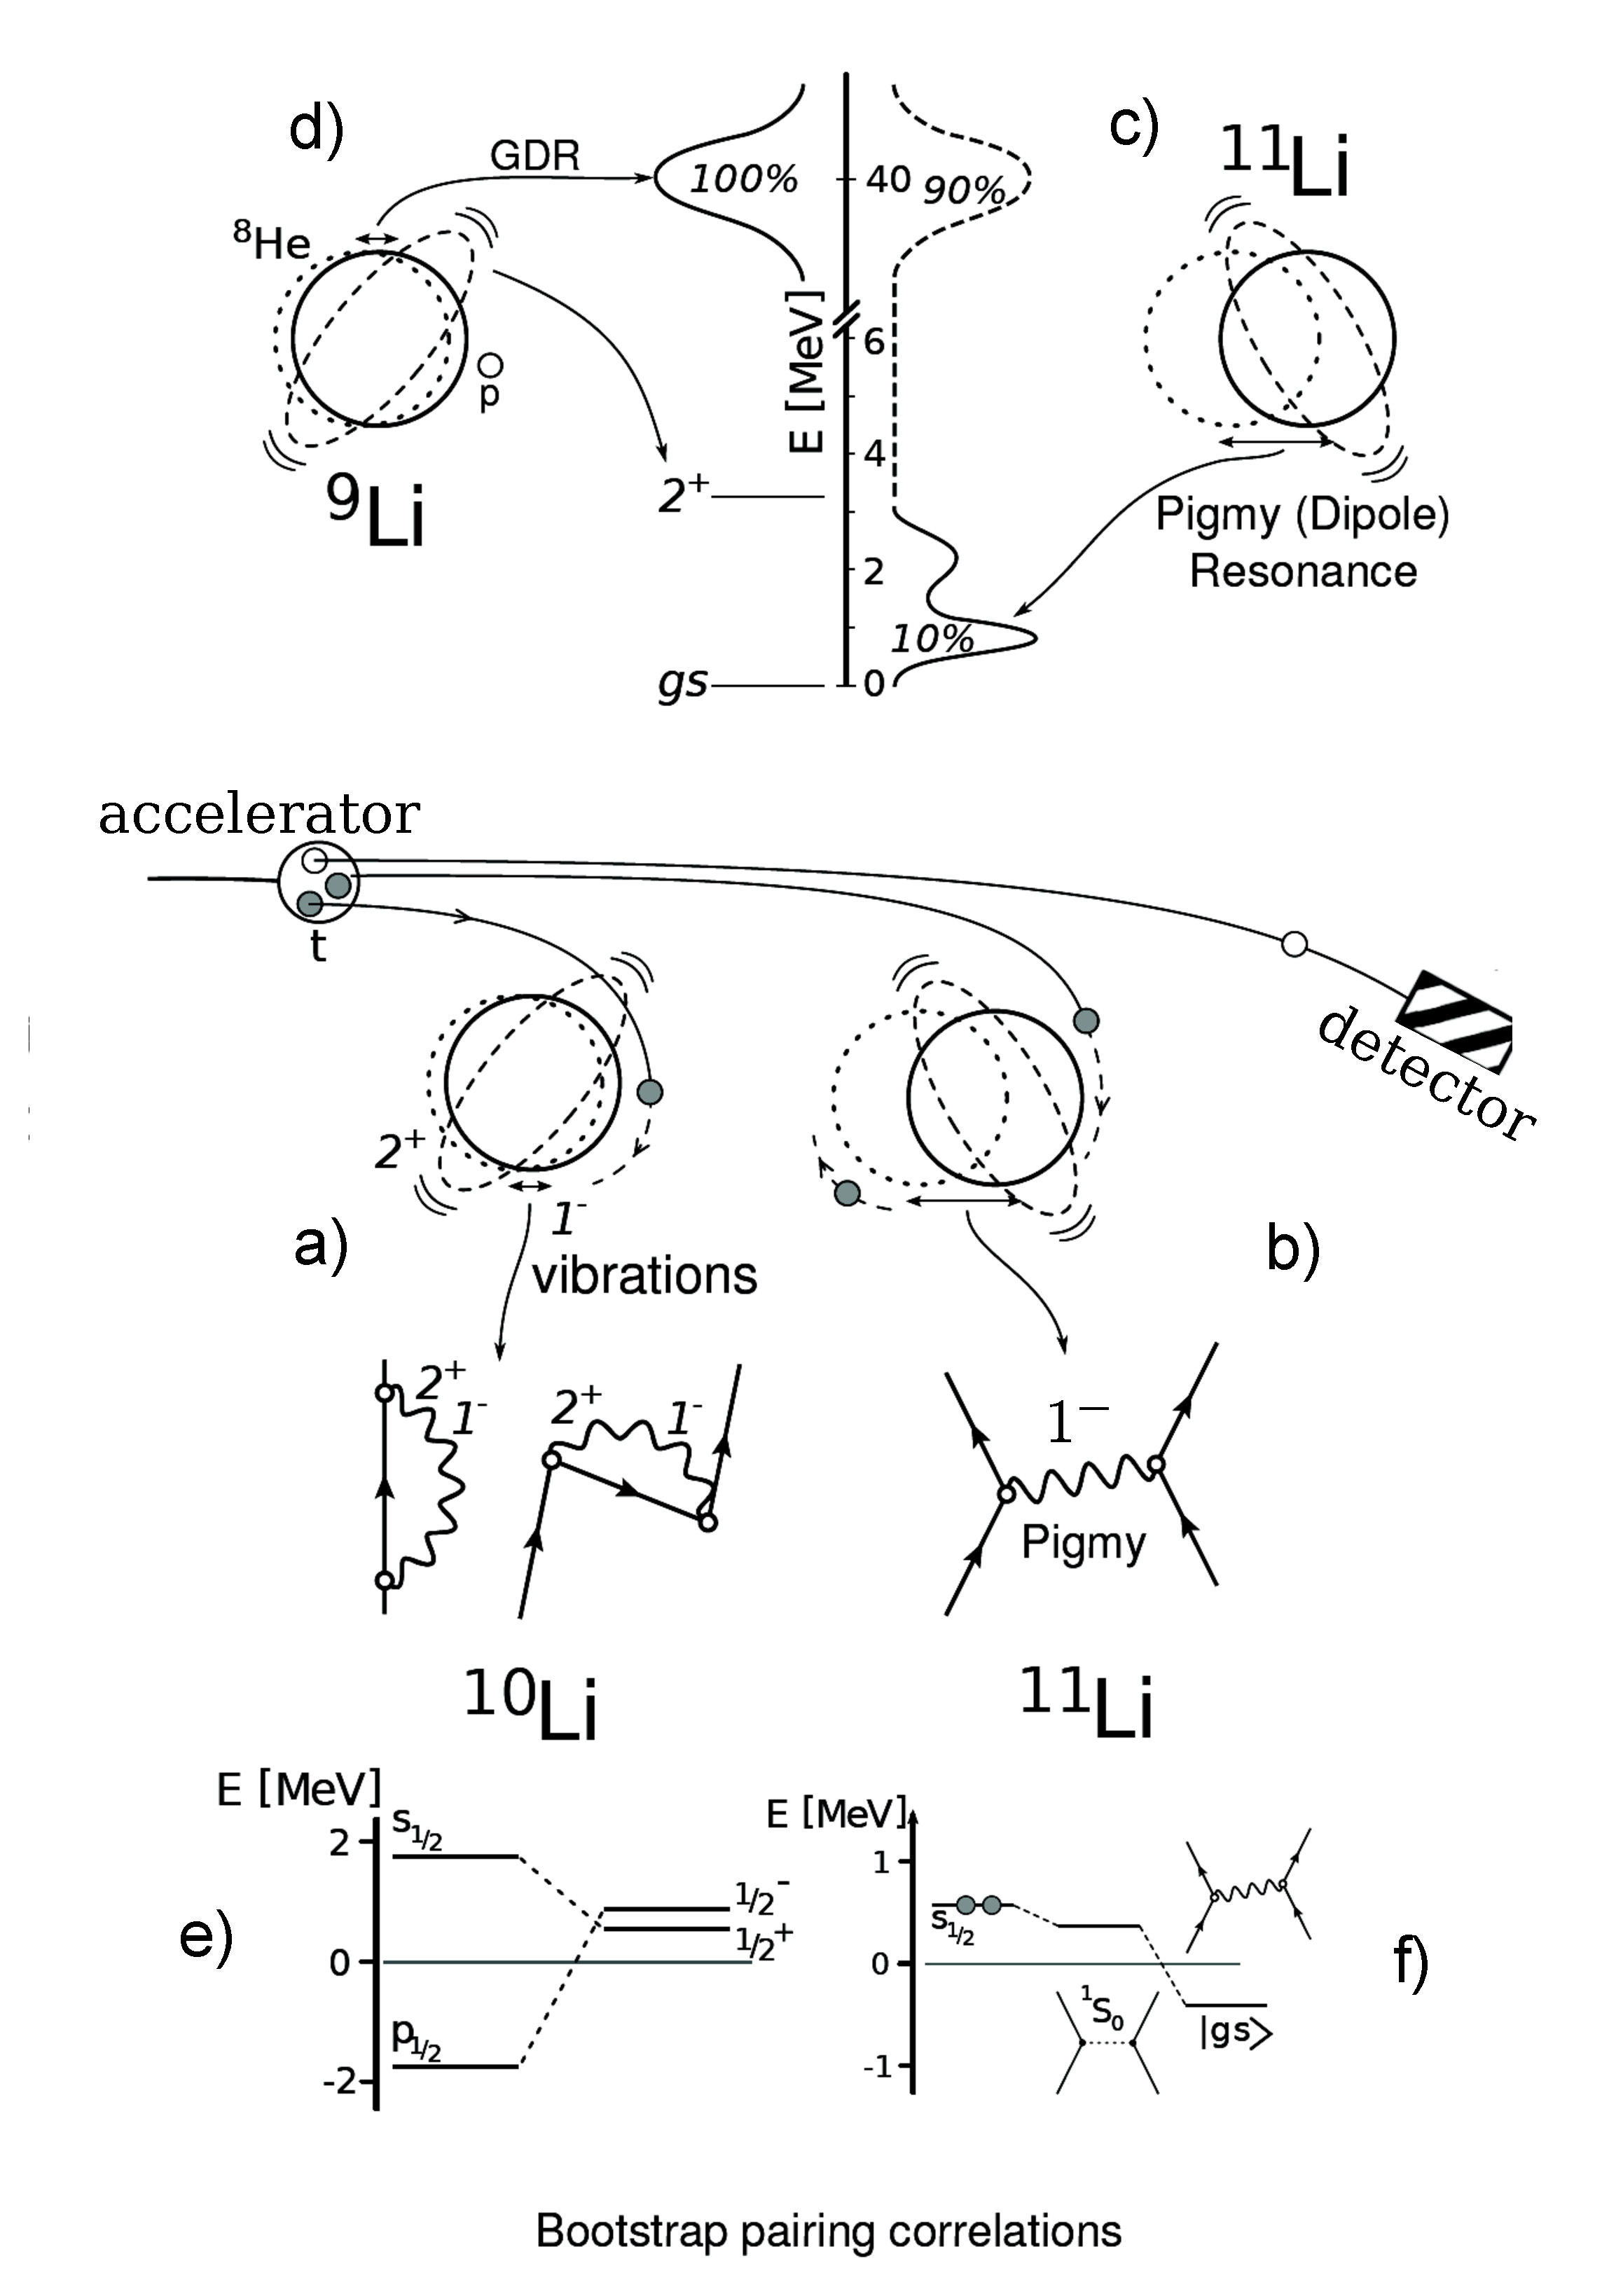
\includegraphics[width=0.75\textwidth]{C8/figsC8/BootStrap_Li}
	\end{center}
	\caption{Schematic representation of the collective quadrupole and dipole response of litium isotopes, and of a ($t,p$) reaction (in the text one reasons in terms of a flux of low energy neutrons) in which two neutrons are transfered to $^9$Li.}
\label{fig8_A_1}
\end{figure}
Such possibility implies that, for a short time, of the order of the traversal time, the two (unbound) neutrons will move in a gas of virtual bosonic excitations, also made out of dipole pygmy resonances. Consequently, they can profit to be almost at threshold by moving in the $\tilde s_{1/2}$ and $\tilde p_{1/2}$ states, to get correlated by exchanging  these bosonic collective vibrations. 
The first phenomenon is associated, as discussed above, with phononic backflow (Pauli principle upflow) leading to $^{10}$Li-like quasi-bound ($s-$wave) and resonant ($p-$wave) dressed single-particle states displaying parity inversion.
The second phenomenon, mediated by phonon exchange between halo neutrons, contributes in a major way to the glue which binds the neutron halo Cooper pair to the $^{9}$Li core. Within the above scenario, one can posit that the $^{11}$Li dipole pygmy resonance can hardly be viewed but in symbiosis with the $^9$Li halo neutron pair addition mode. The above described bootstrap phonon-exchange mechanism can be considered as a novel microscopic embodiment of the Bardeen--Pines--Fr\"{o}lich-like processes to spontaneously break gauge invariance\footnote{Bootstrapping or booting. The term is often attributed to Rudolf Erich Raspe's story The surprising Adventures of Baron M\=unchausen, where the main character pulls himself out of a swamp by his hair. Early 19th century USA: ``pull oneself over a fence by one's bootstraps''}.


To conclude, let us comment on Fig. \ref{fig8_A_1}. As said above, (a) the dressing of single--particle levels by collective vibrations and (b) the renormalization of the bare $NN$--interaction, in particular of the pairing interaction, through the exchange of collective modes between nucleons moving in time reversal states lying close to the Fermi energy, play a central role in nuclear structure. In particular, in the case of the single Cooper pair system $^{11}$Li, most of the glue is provided by the exchange of the dipole pygmy resonance. The pygmy resonance is a chunk of the GDR  and arises from radial inhomogeneous damping. This phenomenon, which arises from extreme neutron excess, is responsible for the isoscalar character\footnote{\cite{Kanungo:15}.} of an antenna--like mode between protons and neutrons\footnote{Similar situations are well known in the case of isoscalar and isovector giant quadrupole resonances (see e.g. \cite{Bes:75c} and references therein).}.   





\section{Alternative processes to populate $\ket{^9\text{Li}(1/2^-)}$}\label{C8AppB}
The $1/2^-$ (2.69 MeV) first excited state of $^9$Li can in principle, not only be populated through a two--particle transfer process, but also through a break up process in which one (see Fig. \ref{fig8_B_1}(a)), or both neutrons (Fig. \ref{fig8_B_1}(b)) are forced into the continuum for then eventually one of them fall into the $1p_{3/2}$ orbital of $^9$Li and excite the quadrupole vibration of the core\footnote{\cite{Potel:10}.}, in keeping with the fact that the main RPA amplitude of this state is precisely $X(1p^{-1}_{3/2},1p_{1/2})(\approx 1)$\footnote{\cite{Barranco:01}.}. The remaining channel populating the first excited state of $^9$Li is associated with an inelastic process (Fig. \ref{fig8_B_1}(c)): two--particle transfer to the ground state of $^{9}$Li and Final State Interaction (FSI) between the outgoing triton and $^{9}$Li in its ground state, resulting in the inelastic excitation of  the $1/2^-$ state.


Making use of the NFT spectroscopic amplitudes, and of a software developed  to take into account microscopically  the different processes mentioned above, that is 9 different reaction channels and continuum states up to 50 MeV of excitation energy, the corresponding transfer amplitudes and associated probabilities $p_l$ were calculated.
 In Table \ref{tab8_B_1} are displayed the probabilities $p_l=|S_l^{(c)}|^2$ associated with each of the processes mentioned above, where the amplitude $S_l^{(c)}$ is related to the total cross section associated with each of the channels $c$  by the expression\footnote{\cite{Satchler:80,Landau:81}.}
\begin{equation}\label{eq6B1}
    \sigma_c=\frac{\pi}{k^2}\sum_l(2l+1)|S_l^{(c)}|^2,
\end{equation}
$k$ being the wave number of the relative motion between the reacting nuclei.



%%
 In keeping with the small values of $p_l$, in what follows we take into account the interference between the contributions associated with the different reaction paths making use of second order perturbation theory, instead of a coupled channel treatment\footnote{See e.g.  \cite{Ascuitto:69} \cite{Tamura:70} \cite{Khoa:04} \cite{Keeley:07b} \cite{Thompson:88}.}. In particular, in the case of the $1/2^-$ (2.69 MeV) first excited state of $^9$Li,
\begin{equation}
    \frac{d\sigma}{d\Omega}(\theta)=\frac{\mu^2}{16\pi^3\hbar^4}\left|\sum_l(2l+1)P_l(\theta)\sum_{c=2}^5 T^{(c)}_l\right|^2,
\end{equation}
where $\mu$ is the reduced mass and $T^{(c)}_l$ are the transition matrix elements associated with the different channels and for each partial wave of DWBA\footnote{\cite{Satchler:80}.}.

\begin{table}
\begin{center}
\begin{tabular}{|c|c|c|c|c|c|}
\hline
\backslashbox {$l$}{$c$} & \textbf{1} & \textbf{2} & \textbf{3} & \textbf{4}& \textbf{5} \\
\hline
 0& $4.35\times 10^{-3}$ &$1.79\times 10^{-4}$ & $4.81\times 10^{-6}$& $2.90\times 10^{-11}$& $3.79\times 10^{-8}$\\
\hline
 1& $3.50\times 10^{-3}$& $9.31\times 10^{-4}$& $1.47\times 10^{-5}$&$1.87\times 10^{-9}$& $1.09\times 10^{-6}$\\
\hline
 2& $7.50 \times 10^{-4}$& $8.00\times 10^{-5}$& $2.45\times 10^{-5}$&$1.25\times 10^{-8}$&$1.21\times 10^{-6}$\\
\hline
 3& $6.12\times 10^{-4}$&$9.81\times 10^{-5}$ & $1.51\times 10^{-6}$&$6.50\times 10^{-10}$&$2.20\times 10^{-7}$\\
\hline
 4&$1.10\times 10^{-4}$ &$ 1.18\times 10^{-5}$ & $2.21\times 10^{-7}$&$4.80\times 10^{-11}$&$1.46\times 10^{-8}$ \\
\hline
 5& $3.65\times 10^{-5}$& $2.16\times 10^{-7}$& $7.42\times 10^{-9}$&$6.69\times 10^{-13}$&$9.63\times 10^{-10}$\\
\hline
 6& $1.35\times 10^{-5}$& $6.05\times 10^{-8}$&$2.88\times 10^{-10}$ &$8.04\times 10^{-15}$&$1.08\times 10^{-11}$\\
\hline
 7& $4.93\times 10^{-6}$& $7.78\times 10^{-8}$& $6.01\times 10^{-11}$&$4.05\times 10^{-16}$&$5.26\times 10^{-13}$\\
\hline
 8& $2.43\times 10^{-6}$& $2.62\times 10^{-8}$& $7.4\times 10^{-12}$&$1.26\times 10^{-17}$&$9.70\times 10^{-11}$\\
\hline
\end{tabular}
\caption{Probabilities $p_l$  associated with the processes described in the text for each partial wave $l$. The different channels are labeled by a channel number $c$ equal to: \textbf{1}, multistep transfer to the $^9$Li ground state (Fig. \ref{fig8_B_1}(d)); \textbf{2}, multistep transfer (Fig. \ref{fig8_B_1}(e)) to the first excited $^9$Li state, \textbf{3}, breakup (Fig. \ref{fig8_B_1}(f)), \textbf{4}, breakup  (Fig. \ref{fig8_B_1}(g)), and \textbf{5} inelastic processes (Fig. \ref{fig8_B_1}(h)) involved in the population of the $1/2^-$ (2.69 MeV) first excited state of $^9$Li. It is of notice that the probabilities displayed in columns \textbf{1} and \textbf{2} result from the (coherent) sum of three amplitudes namely those associated with successive, simultaneous and non--orthogonality transfer channels (see also Figs. \ref{fig8_B_2} and \ref{fig8_B_3}) after \cite{Potel:10}.}\label{tab8_B_1}
\end{center}
\end{table}


 Making use of all the elements discussed above, multistep transfer\footnote{\cite{Bayman:82}, \cite{Igarashi:91},  \cite{Bayman:73} as well as \cite{Broglia:04a}.}, breakup and inelastic channels were calculated, and the results displayed in Figs. \ref{fig8_B_2} and \ref{fig8_B_3} and in Table \ref{tab8_B_1}. Theory provides an overall account of the experimental findings. In particular, in connection with the $1/2^-$ state, this result essentially emerges from cancellations and coherence effects taking place between the three terms contributing to the multistep two--particle transfer cross section (Fig. \ref{fig8_B_3}), tuned by the nuclear structure amplitudes associated with the process shown in Fig. \ref{fig8_B_1} (e) as well as Eqs. (\ref{eq8_2_1})--(\ref{eq8_2_3}). In fact, and
as shown in Figs. \ref{fig8_B_2} and \ref{fig8_B_3}, the contributions of break up processes and inelastic   (Figs. \ref{fig8_B_1}(f),(g) and (h) respectively) to the population of the $1/2^-$ (2.69 MeV) first excited state of $^9$Li are negligible as compared with the process depicted in Fig. \ref{fig8_B_1}(e). In the case of the breakup channel (Figs. \ref{fig8_B_1}(f) and \ref{fig8_B_1}(g)) this is a consequence of the low bombarding energy of the $^{11}$Li beam (inverse kinematics), combined with the small overlap between continuum (resonant) neutron $p_{1/2}$ wavefunctions and  bound state wavefunctions. In the case of the inelastic process (Fig. \ref{fig8_B_1}(h)), it is again a consequence of the relative low bombarding energy. In fact, the adiabaticity parameters $\xi_C,\xi_N$\footnote{See eqs. (IV.12) and (IV.14) of ref. \cite{Broglia:04a}.} associated with Coulomb excitation and inelastic excitation in the t+$^9$Li channel are larger than 1, implying an adiabatic cutoff. In other words, the quadrupole mode is essentially only polarized during the reaction but not excited. The situation is quite different in the case of the intervening of the virtual processes  displayed in Fig. \ref{fig8_B_1} (b) and (c) leading to the population of the $1/2^-$ state displayed in Fig. \ref{fig8_B_1} (e). Being those off--the--energy shell processes, energy is not conserved, and adiabaticity gets profoundly modified.

  \begin{figure}
  \centerline{\includegraphics*[width=12cm,angle=0]{C8/figsC8/fig8_B_1x}}
  	\caption{Representative Nuclear Field Theory--Feynman diagrams associated with correlation process ((a),(b),(c)) and with one-- and two--particle pick--up reactions ((i),(j) and (d),(e) respectively) of the halo neutrons of $^{11}$Li (Cooper pair, indicated in terms of a double arrowed line). Also shown are the possible diagrams associated with other channels (breakup and inelastic) populating the $1/2^-$ (2.69 MeV) state: f) two--particle pickup reaction involving one of the halo neutrons (the other one going into the continuum, i.e. breaking up from the $^9$Li core) together with a neutron from the $p_{3/2}$ orbital of the $^9$Li core  leading eventually to the excitation of the $1/2^-$ final state ($2^+$ density mode (wavy line) coupled to the $p_{3/2}(\pi)$), g) the proton field acting once breaks the Cooper pair forcing one of the halo neutrons to populate a $p_{1/2}$ continuum state (the other one follows suit), while acting for the second time picks up one of the neutrons moving in the continuum and another one from those moving in the $p_{3/2}$ orbital of $^9$Li eventually leaving the core in the quadrupole mode of excitation. In (h) the  two--step transfer to the $^9$Li ground state plus the inelastic final channel process exciting the $(2^+\otimes p_{3/2}(\pi))_{1/2^-}$ state is shown. After \cite{Potel:10}.}\label{fig8_B_1}
  \end{figure}
    \begin{figure}
    \centerline{\includegraphics*[width=12cm,angle=0]{C8/figsC8/fig8_B_2}}
    	\caption{Experimental (\cite{Tanihata:08}) and theoretical differential cross sections (including multistep transfer as well as breakup and inelastic channels, \cite{Potel:10})  of the
    	$^1$H($^{11}$Li,$^9$Li)$^3$H  reaction populating the ground state ($3/2^-$) and the first excited state ($1/2^-$; 2.69 MeV) of $^{9}$Li. Also shown (dash--dotted curve) is the differential cross section associated with this last state but taking into account only multistep transfer. The optical potentials used are from \citep{Tanihata:08,An:06}, see Table \ref{tab8.1.1}. The absolute cross sections associated with the ground state ($3/2^-$) is predicted to be 6.1 mb (exp: $5.7\pm 0.9$ mb) while that corresponding to the first excited state ($1/2^-; 2.69$ MeV) being 0.7 mb (exp: $1.0\pm 0.36$ mb). }\label{fig8_B_2}
    \end{figure}
        \begin{figure}
        \centerline{\includegraphics*[width=12cm,angle=0]{C8/figsC8/fig8_B_3}}
        	\caption{Successive, simultaneous and non-orthogonality contributions (prior representation)
        	to the  $^1$H($^{11}$Li,$^9$Li)$^3$H differential cross section
        	associated with the population of the $1/2^-$ state
        	of $^9$Li, displayed in Fig. \ref{fig8_B_2}. Also shown is the (coherent) sum of the breakup ($c=3$ and 4) and inelastic ($c=5$) channel contributions.}\label{fig8_B_3}
        \end{figure}

\section{Software}\label{C8AppD}
In this Appendix we provide a brief description of the numerical methods implemented in the code written to evaluate the differential cross sections. The two--nucleon transfer differential cross section is given by Eq. (\ref{eq5.1.4}),  so the principal task consist in calculating the transfer amplitudes $T^{(1)}(\theta),T^{(2)}_{succ}(\theta)$ and $T^{(2)}_{NO}(\theta)$ described in Eqs. \ref{eq1_40}--\ref{eq1_42}, by numerically evaluating the corresponding integrals.  The dimensionality of the integrals  can be reduced by expanding in partial waves (eigenfunctions of the angular momentum operator) the distorted waves and wavefunctions present in the corresponding integrands. The resulting expressions are Eqs. (\ref{eq111}) and (\ref{eq112}) for $T^{(1)}(\theta)$, Eqs. (\ref{eq27}), (\ref{eq121}) and (\ref{eq122}) for $T^{(2)}_{succ}(\theta)$, and Eqs. (\ref{eq138}), (\ref{eq139}) and (\ref{eq140}) for $T^{(2)}_{NO}(\theta)$. The integrals are computed numerically with the method of Gaussian quadratures. 


The one--dimensional (radial) functions appearing in the integrands are defined in a spatial grid up to a given maximum radius $r_{max}$. The bound state  wavefunctions are obtained by numerical integration of the radial Schr\"odinger equation for a Woods--Saxon potential with a spin--orbit term. The parameters defining the shape of the potential are given as an input, while the depth is adjusted to reproduce the binding energy of the state under consideration. The resulting potential corresponding to the final (initial) nucleon bound state stands also for the interaction potential featured in the integrand in the prior (post) representation. The distorted waves are obtained by integrating the radial Schr\"odinger equation with positive energy from $r=0$ to $r_{max}$, and matching the solution with the corresponding Coulomb wave function at a given $r=r_{match}$, big enough to lie outside of the range of the nuclear interaction. The  Woods--Saxon optical potentials  used to obtain the distorted waves consist on a real Coulomb term, a real and imaginary volume terms, an imaginary surface term, and a real and imaginary spin orbit terms. The parameters needed to specify all those terms are given as an input.  




   

\section{Statistics.}\label{App6D}
Let us consider two identical particles moving in a one--dimensional harmonic oscillator. Let us assume  that one is in the ground state and the other  is in the first excited state. According to the superposition principle 
\begin{align}\label{eqApp6G1}
\Phi(x_1,x_2)=\lambda\phi_1(x_1)\phi_0(x_2)+\mu\phi_0(x_1)\phi_1(x_2).
\end{align} 
Let us calculate the correlation of these particles, that is, the quantity
\begin{align}\label{eqApp6G2}
Corr=\frac{\langle x_1x_2\rangle-\langle x_1\rangle\langle x_2\rangle}{\sqrt{\left(\langle x_1^2\rangle-\langle x_1\rangle^2\right)\left(\langle x_2^2\rangle-\langle x_2\rangle^2\right)}}
\end{align} 
Let us start with
\begin{align}\label{eqApp63}
\nonumber\langle x_1x_2\rangle=&\int dx_1 dx_2 \left(\lambda^*\phi_1^*(x_1)\phi_0^*(x_2)+\mu^*\phi_0^*(x_1)\phi_1^*(x_2)\right)\\
\nonumber&\times(x_1 x_2)\left(\lambda\phi_1(x_1)\phi_0(x_2)+\mu\phi_0(x_1)\phi_1(x_2)\right)\\
\nonumber &=|\lambda|^2\langle\phi_1|x_1|\phi_1\rangle\langle\phi_0|x_2|\phi_0\rangle+\lambda^*\mu\langle\phi_1|x_1|\phi_0\rangle\langle\phi_0|x_2|\phi_1\rangle\\
&+\lambda\mu^*\langle\phi_0|x_1|\phi_1\rangle\langle\phi_1|x_2|\phi_0\rangle+|\mu|^2\langle\phi_0|x_1|\phi_0\rangle\langle\phi_1|x_1|\phi_1\rangle\langle\phi_0|x_1|\phi_0\rangle\langle\phi_1|x_1|\phi_1\rangle.
\end{align} 

In keeping with the fact that

\begin{align}\label{eqApp6G4}
\langle\phi_1|x|\phi_1\rangle=\langle\phi_0|x|\phi_0\rangle=0,
\end{align} 
and
\begin{align}\label{eqApp6G5}
\langle\phi_0|x|\phi_1\rangle=\langle\phi_1|x|\phi_0\rangle=\sqrt{\frac{\hbar\omega}{2C}},
\end{align}
one obtains
\begin{align}\label{eqApp6G6}
\langle x_1x_2\rangle=\left(\frac{\hbar\omega}{2C}\right)\Re(\lambda^*\mu).
\end{align} 
And 
\begin{align}\label{eqApp6G7}
\sqrt{\quad}=\left(\frac{\hbar\omega}{2C}\right),
\end{align}
for the denominator of Eq. (\ref{eqApp6G2}).
From the above results the correlation function between particle 1 and 2 is
\begin{align}\label{eqApp6G8}
Corr=\frac{2C}{\hbar\omega}\langle x_1x_2\rangle=2\Re(\lambda^*\mu)=
\left\{
\begin{array}{c}
 1\quad (\lambda=+\mu=\frac{1}{\sqrt{2}})\\ 
 -1 \quad (\lambda=-\mu=\frac{1}{\sqrt{2}})
\end{array}
\right. 
\end{align}
It is of notice that, in quantum mechanics, average values imply the mean outcome of a large number of experiments. In this case, of the (simultaneous) measure of the position of the two particles\footnote{\cite{Basdevant:05}.}.






\section{Correlation length and quantality parameter.}\label{App6H}
The correlation length can be defined as\footnote{See e.g. \cite{Annett:13} p. 62.}
\begin{align}\label{eqApp6H1}
\xi=\frac{\hbar v_F}{\pi\Delta}\approx\frac{\hbar^2}{m}\frac{k_F}{\pi\Delta}
\end{align}
where the Fermi momentum in the case of stable nuclei lying along the stability valley is
\begin{align}\label{eqApp6H2}
k_F\approx 1.36\,\text{fm}^{-1}.
\end{align}
Thus,
\begin{align}\label{eqApp6H3} 	
\xi=40\,\text{MeV fm}^2\times \frac{1.36}{\pi\Delta}\,\text{fm}^{-1}\approx \frac{17}{\Delta}\,\text{fm},
\end{align}
and,
\begin{align}\label{eqApp6H4}
\xi\approx 14\,\text{fm},\quad (\Delta\approx1.2\,\text{MeV}).
\end{align}
Thus, the associated (generalized) quantality parameter is, in the present case,
\begin{align}\label{eqApp6H8}
q_\xi=\frac{\hbar^2}{2m\xi^2}\frac{1}{2\Delta}\approx0.04.
\end{align} 
That is, the two partner nucleons are, in the Cooper pair, rigidly correlated with each other.
We now consider $^{11}$Li, and calculate $k_F$ (neutrons) with the help of the Thomas--Fermi model\footnote{Quantity which can be related to ($v_F/c$) according to the relation ($v_F/c)=\hbar k_F/(mc)=(\hbar c/(mc^2))k_F\approx0.2(k_F){\text{fm}^{-1}}$). In the case in which $k_F\approx 0.8 $ fm$^{-1}$ (see Eq. (\ref{eqApp6H9})) to $v_F/c\approx 0.16$. }
\begin{align}\label{eqApp6H9}
k_F=\left(3\pi^2\frac{8}{\frac{4\pi}{3}(4.58)^3}\right)^{1/3}\,\text{fm}^{-1}\approx\frac{(18\pi)^{1/3}}{4.58}\,\text{fm}^{-1}\approx 0.8\,\text{fm}^{-1}.
\end{align} 
The correlation length can, in the present case, be calculated in terms of the correlation energy ($E_{corr}\approx-0.5$ MeV), 
\begin{align}
\xi\approx \frac{\hbar v_F}{\pi|E_{corr}|}\approx \frac{20 \text{ MeVfm}\times0.16}{\pi\times 0.5\text{ MeV}}\approx 20\text{ fm},
\end{align}
 the resulting generalized quantality parameter being
\begin{align}\label{eqApp6H13}
q_\xi=\frac{\hbar^2}{2m\xi^2}\frac{1}{|E_{corr}|}\approx 0.1.
\end{align}
It is of notice that this result is but an alternative embodiment of the relation (\ref{eq3.3.8}). Now, one could argue that both (\ref{eq3.3.8}) and (\ref{eqApp6H13}) (as well as (\ref{eqApp6H8}) for stable nuclei), are just a manifestation of (\ref{eqApp6G8}). That there is more to it is forcefully expressed by the fact that, selecting the pure two--particle configuration $|s_{1/2}^2(0)\rangle$ ($|p_{1/2}^2(0)\rangle$) to describe the halo neutron Cooper pair of $^{11}$Li leads to absolute two--particle transfer cross sections which are about one order of magnitude larger (smaller) than the observed cross section (see Fig. \ref{fig8_1_2}). The fact that the NFT result (\ref{eq8_2_1})--(\ref{eq8_2_3}) with its unusual pygmy binding and quadrupole driven parity inversion clothing mechanism reproduces observations within experimental errors, underscores the central role played by structure on Cooper pair tunneling, through the emergent property of generalized pairing rigidity.


Summing up, both bare $NN$-- and long range induced pairing interaction changes the statistics of the elementary modes from fermionic to (quasi) bosonic ones\footnote{Within this context see Sect. \ref{C3AppD}.} and, at the same time, the value of the quantality parameter from $q\approx1$ to $q_\xi\ll 1$, thus  from a regime of delocalized single nucleons to one of strongly overlapping, independent pair motion each being governed by the same phased wavefunction ($U'_{\nu}+V'_{\nu}e^{-2i\phi}P^\dagger_\nu)\ket{0}$, where $P^\dagger_\nu=a^\dagger_\nu a^\dagger_{\hat\nu}$ create two nucleons in time reversal states\footnote{Since $P^\dagger_\nu$ commutes for different $\nu$'s, $\ket{BCS}$ represents uncorrelated occupancy of the various pair states.}. In each pair, the partners are phase correlated to each other (see Eq. (\ref{eq3.2.19})) behaving as a single entity. The operator $P^\dagger_\nu$, being a product of two fermions, do not fulfill Bose statistics ($(P^\dagger_\nu)^2=0$). This property implies the presence of a pairing gap not only for breaking a pair, but also for making a pair move differently from the others\footnote{The BCS state can be written as $\ket{BCS}\sim\Pi_\nu \alpha_\nu\ket{0}$, where $\alpha_\nu=U_\nu a_\nu-V_\nu a^\dagger_{\hat{\nu}}$, is the annihilation quasiparticle operator (\cite{Bogoljubov:58,Valatin:58}; see App. G of \cite{Brink:05}). Thus, to make a pair which occupies the state $\nu'$ to behave differently from the rest of the pairs one has to avoid including in the product above the state $\nu'$, i.e. $\Pi_{\nu\neq\nu'} \alpha_\nu\ket{0}$. The resulting state resembles a one--quasiparticle state.}. As a result one has long--range--order in the superfluid nuclear system, known as off--diagonal--long--range--order (ODLRO)\footnote{\cite{Yang:62}.}.  This effect leads  to  generalized gauge rigidity, the detailed renormalizing and dressing mechanisms ultimately deciding on the soundness and applicability of the description under discussion. The fact that in working out the reaction mechanism one uses, for practical reasons, a single--particle basis (second order DWBA corrected by non--orthogonality), reconstructing the pair correlations in term of sums over virtual states, is at the basis of the two--neutron transfer physical sum rule discussed in Sect. \ref{S6.4.2}.
 


\section{Multipole pairing vibrations.}\label{App6G}
\begin{figure}
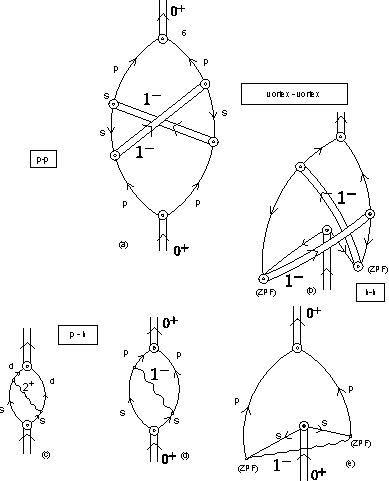
\includegraphics[width=\textwidth]{C8/figsC8/figA1_corr.pdf}
\caption{ NFT-Feynman diagrams describing the interweaving between the neutron halo pair addition monopole and dipole modes
(double arrowed lines labeled $0^+$ and $1^-$ respectively). Above, the exchange of dipole modes binding the $0^+$ pair addition mode through  forwards going particle-particle p-p (h-h) components. Below,  the assumption is made that the GDPR of $^{11}$Li can be viewed as a p-h (two quasiparticle), QRPA mode.}\label{fig6.I.1}
\end{figure}

\begin{figure}
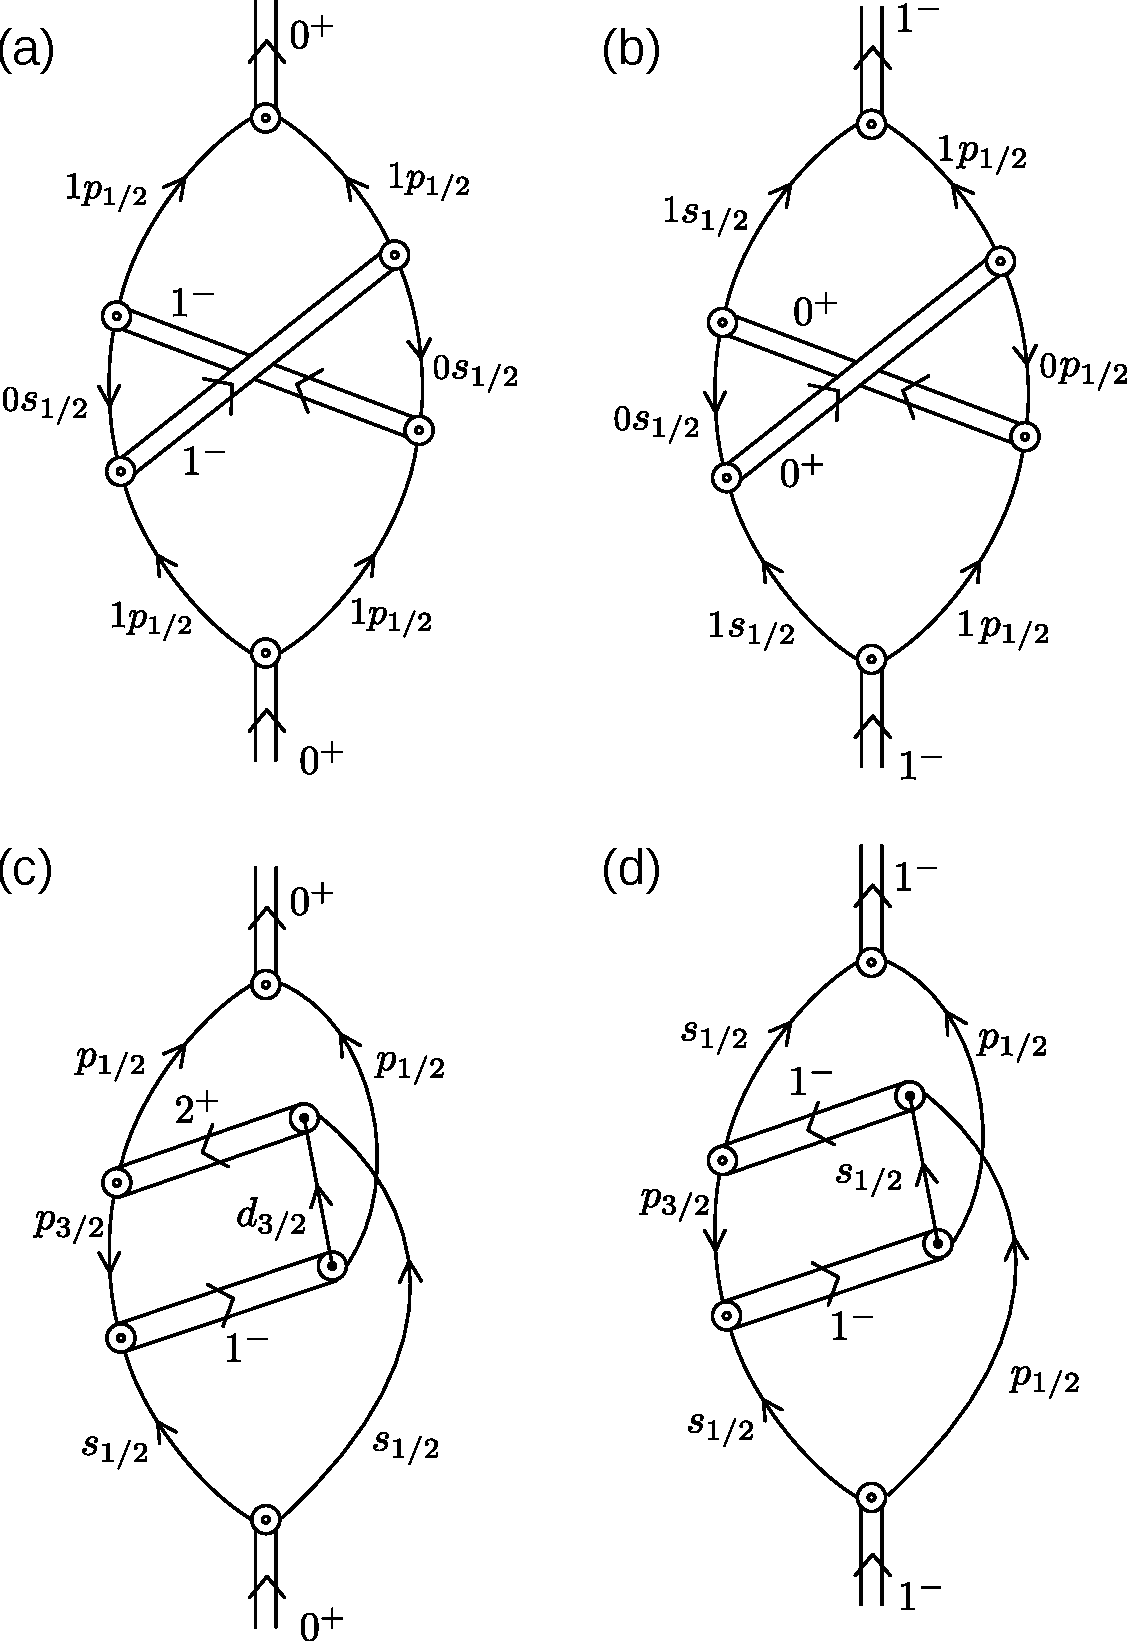
\includegraphics[width=0.8\textwidth]{C8/figsC8/Nobel40Years-4b.pdf}
\caption{NFT-Feynman diagrams describing, (a,c) some of the particle-particle (pp),hh and ph processes binding the Cooper pair neutron halo 
and stabilizing $^{11}$Li, as well as  (b,d) giving rise to the GDPR.}\label{fig6.I.2}
\end{figure}

\begin{figure}
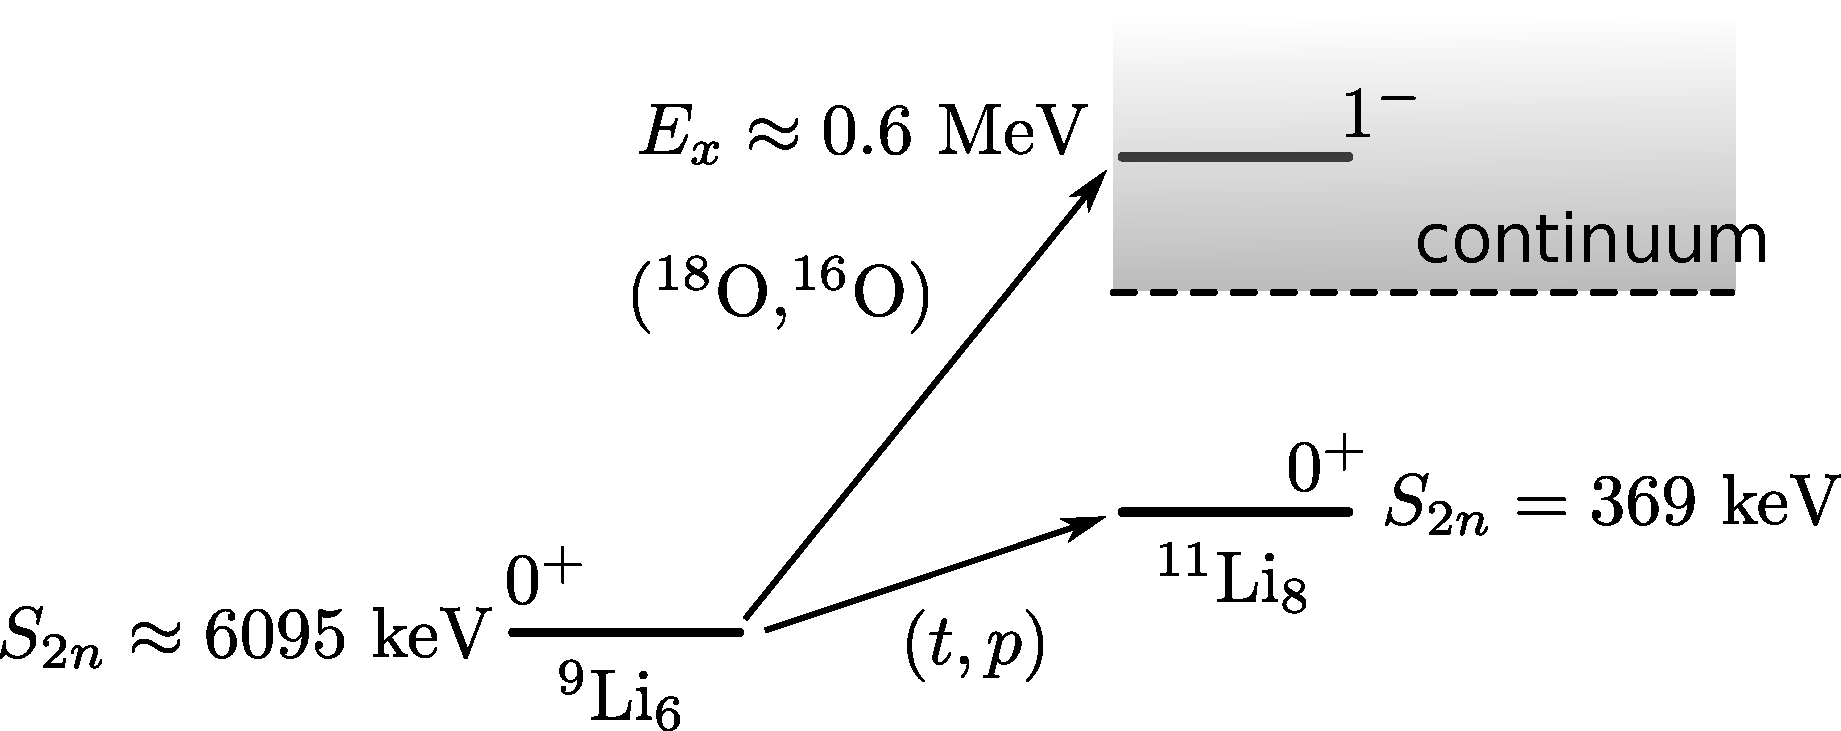
\includegraphics[width=\textwidth]{C8/figsC8/figa3_newnew.pdf}
\caption{ Schematic representation of levels of $^{11}$Li populated (gs), or which  eventually could be populated ($1^-$)  in two--nucleon transfer reactions. Indicated in keV are the two--neutron
separation energies $S_{2n}$. In labeling the different states, one has not considered the quantum numbers of the $p_{3/2}$ odd proton. }\label{fig6.I.3} 
\end{figure}

\begin{figure}
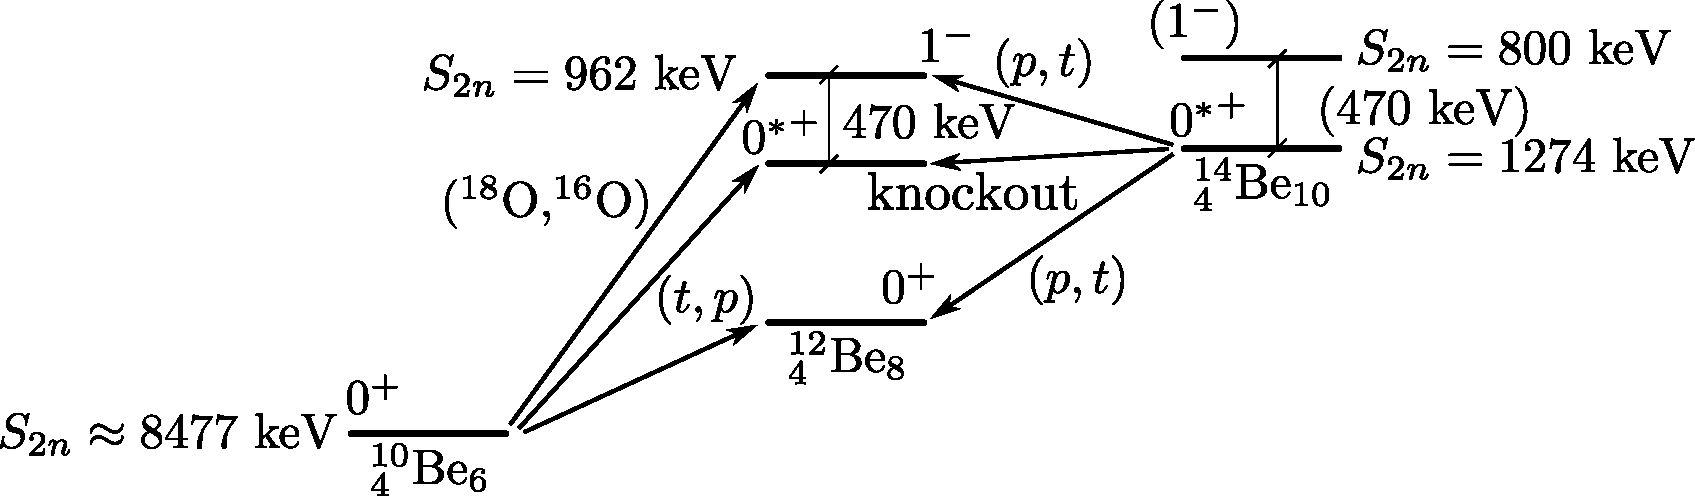
\includegraphics[width=\textwidth]{C8/figsC8/figa4_newnew.pdf}
\caption{Levels of $^{12}$Be expected to be populated in two-nucleon transfer and knockout processes. $S_{2n}$ are the two-neutron separation energies.}\label{fig6.I.4}
\end{figure}




Although much work has been carried out concerning multipole pairing vibrations\footnote{See \cite{Brink:05} Sect. 5.3 and refs. therein. See also  \cite{Broglia:74}, \cite{Ragnarsson:76}, \cite{Broglia:71b}, \cite{Broglia:71c}, \cite{Bes:71d}, \cite{Bes:71}, \cite{Flynn:71}, \cite{Bes:72}, \cite{Broglia:81c}, \cite{Bohr:74b}, \cite{Flynn:72},  \cite{Bortignon:76}; see also \cite{Kubo:70} and references therein.}, i.e. modes with transfer quantum numbers $\beta=\pm2$ and multipolarity and parity $\lambda^\pi$ different from $0^+$, this remains a chapter essentially missing from the subject of pairing in nuclei. Arguably, with the partial exception of quadrupole pairing studied in the multiphonon pairing vibrational spectrum\footnote{See \cite{Flynn:72}.} around the closed shell $^{208}$Pb, and in connection with strongly excited $0^+$ pairing vibrational states in the actinide region\footnote{\cite{Casten:72}, \cite{Bes:72}, \cite{Ragnarsson:76}. It is of notice that $\beta$--vibrations and monopole pairing vibrations become mixed in quadrupole deformed nuclei.}, as well as of the quadrupole and hexadecapole pairing vibrations in the multiplet spectrum\footnote{\cite{Bortignon:76}.} of $^{209}$Bi.

In what follows, we shall elaborate on the new insight on pairing vibrational modes, the studies of two--neutron pickup reactions on $^{11}$Li have opened. As already explained, because of the small overlap existing between halo neutrons and core nucleons both the $^1S_0$, NN- and the symmetry-potential become strongly screened, resulting in a subcritical value of pairing strength and in a weak repulsion to separate protons from neutrons in the dipole channel.
As a result, neither the $J^{\pi}=0^+$ correlated neutron state  (Cooper pair), nor the $J^\pi=1^-$ one (vortex--like)\footnote{One of the effects of a vortex is that it allows rotation about an axis of symmetry.} are bound 
(although both qualify to do so) to the core $^{9}$Li. 


Having essentially exhausted the bare NN-interaction channels, the two neutrons can correlate their motion by exchanging vibrations of the medium in which they propagate, namely  the halo and the core. Concerning the first one, these modes could hardly  be the $\lambda= 2^+,3^-$ or $5^-$ surface vibrations found in 
nuclei lying along the  stability valley. This is because the diffusivity of the halo is so large that it blurs the very definition of surface. Those associated with  the core ($ 2^+$ see Fig. \ref{fig6.I.1} (c), and eventually also $3^-,5^-$ etc.) provide some glue, but insufficient to bind any of the two dineutron states in question.

As already mentioned, the next alternative is that of bootstrapping. Namely, that in which the two partners of the  (monopole) Cooper pair exchange  pairs of vortices 
(dipole Cooper pair),  as well as one dipole Cooper pair and a quadrupole pair removal mode,
while those of the vortex exchange  pairs of Coopers pairs (monopole pairing vibrations), but also pairs of dipole pairs, as shown in Figs. \ref{fig6.I.1} and \ref{fig6.I.2}.  In other words, by  liaising  with each other,  
the two dineutrons contenders at the role of $^{11}$Li ground state  settle the issue.  As a result  the Cooper pair becomes weakly bound ($S_{2n}$ = 389 keV), the vortex state remaining barely unbound, by about 0.5-1 MeV.
There is no physical reason why things could not have gone  the other way, at least none that we know. Within this context we refer to $^3$He superfluidity, where condensation involve $S=1$ pairs. It is of notice that we are not considering spin degrees of freedom in  the present case,
at least  not dynamic ones. 

For practical purposes, one can describe the  $1^-$ as a two quasiparticle state and calculate it within  the framework of QRPA adjusting the strength of the dipole-dipole separable interaction to reproduce the  experimental findings (Fig. \ref{fig3C1}). In this basis it is referred to  as a Giant Dipole Pygmy Resonance (GDPR). Exchanged between the  two partners of the Cooper pair (Fig. \ref{fig6.I.1}(d)) leads to essentially the right value of  dineutron binding  to the $^9$Li core. Within this context  one can view the
$^{11}$Li neutron halo as a van der Waals Cooper pair (Fig. \ref{fig6.I.1}(e)). The transformation between this picture and  that discussed in connection with 
(a) and (b) as well as with Fig. \ref{fig6.I.2} can be obtained  expressing the GDPR, QRPA wavefunction, in terms of particle  creation and destruction operators (Bogoliubov-Valatin transformation) as seen from Fig. \ref{fig6.I.1}(a) and (b). 
A vortex-vortex  stabilised Cooper pair emerges. 

Which of the two  pictures is more adequate to describe  the dipole mediated condensation is an open question,  
as each of them reflects  important physical properties which   characterise  the GDPR. In any case, both indicate the symbiotic character  of the halo Cooper pair  addition mode  and of the pygmy resonance  built on top of, and almost degenerate with it. 
Insight into this question can be obtained  by shedding light on the question  of whether  the velocity field of each of the symbiotic  states is more similar  to that associated  with irrotational or vortex--like flow\footnote{See \cite{Repko:13}. Within this context, and making use of an analogy, one can  mention that a consistent description of the GQR and of the GIQR is obtained 
assuming that the average eccentricity of neutron orbits 
is equal to the average eccentricity of the proton orbits (\cite{Bes:75c}), the scenario of neutron skin.
The  isoscalar quadrupole-quadrupole interaction is attractive. Furthermore, 
the valence orbitals of nuclei have, as a rule and aside from intruder states, homogeneous parity. These facts  preclude 
the GQR to play the role of the GDPR. In fact, there will always be a low--lying quadrupole vibration closely 
connected with the aligned coupling scheme and thus  with nuclear plasticity. Within this context one can  nonetheless  posit  that the GQR, related to neutron skin,  is closely associated with the aligned coupling scheme.
Making a parallel, one can posit  that the GDPR is closely connected with vortical motion. 
Arguably,  support for this picture is provided by the   low-lying  E1 
strength of $^{11}$Li. It  results from the presence of $s_{1/2}$ and $p_{1/2}$ orbitals almost degenerate and at threshold, 
leading to a low-lying Cooper pair coupled to angular momentum $1^-$. (dipole pair addition mode). 
The  scenario of vortical motion. }. Two-nucleon transfer reactions, specific probe  of (multipole) pairing vibrational modes, contain many of the answers to the above question (Figs. \ref{fig6.I.3}). 
In fact,  ground state correlations will play a very different role in the absolute value of the $^9$Li(t,p)$^{11}$Li ($1^-$) cross section,
depending  on which picture is correct. In the case in which 
it can be 
 viewed as a vortex (pair addition dipole mode) it will lead to an increase of the two-particle transfer reaction 
 (positive coherence).
 It will  produce the opposite effect if the correct interpretation of the GDPR   is that of a 
($p-h$)--like excitation\footnote{ \cite{Broglia:71}.}. 
Insight  in the above question may also be obtained by studying  the properties of
a quantal vortex in a Wigner cell with parameters which approximately reproduce 
the halo of $^{11}$Li. Within this context, and  for the solely purpose of providing an analogy, we refer 
to what is done in the study of vortices in the environment of neutron stars\footnote{\cite{Avogadro:07,Avogadro:08}.}.


A  possible test of the soundness of the physics  discussed above, concerns the question of whether the first excited, 
$0^+$ halo state ($E_x$= 2.24 MeV) of $^{12}$Be can be viewed as the $|$gs($^{11}$Li$)\rangle$ in a new environment. In other words, 
to consider the halo neutron pair addition mode
 a novel mode of  elementary excitation: neutron halo pair  addition mode of which the $|1^- $($^{12}$Be) ; 2.71 MeV$\rangle $ is 
 a fraction of  its symbiotic  GDPR partner. One can gain insight concerning this question, by 
 eventually measuring the E1-branching ratio $|1^-$ (2.71 MeV)$\rangle  \to |0^+$* (2.24 MeV)$\rangle$ ), and possibly 
 finding other low-energy E1-transitions populating the $0^*$ state, as well as through  two--nucleon stripping process,
 and two--nucleon pickup and knockout reactions (Fig. \ref{fig6.I.4}).
 A resum\'e of the picture discussed above is given   in Fig. \ref{fig3.8.1}. 
 \section{Vacuum fluctuations and interactions: the Casimir effect}






\end{subappendices}
\renewcommand{\bibname}{Bibliography Ch 6}
\bibliographystyle{abbrvnat}
%\bibliography{C:/Gregory/Broglia/notas_ricardo/nuclear_bib}
 \bibliography{../nuclear_bib}